%!TEX root = paper.tex
\section{Evaluation}
\label{sec:results}

In this section, we present insights about the distinguishability of the devices in the wild based on their hardware imperfections, by collecting a large dataset of BLE signals transmitted by commercial devices in use. We evaluate the feasibility of RF fingerprinting in the wild and elaborate upon the aforementioned challenges and limitations of RF fingerprinting using our field data.


% \subsection{The choice of receiver}
% Our RF fingerprinting attack begins by capturing the BLE signals on the air using a Software Defined Radio (SDR). The first question that naturally rises is whether the choice of the SDR significantly affects the accuracy of our attack. In other words, \textit{can we use an inexpensive receiver such as LimeSDR-Mini to deploy such attack?} In fact the accuracy of our attack is dependent on the quality of the received signal and the extracted hardware imperfections. To show that the quality of the estimated hardware imperfections remains the same even if we capture with a less expensive receiver, we send packets from an iPhone device and capture the signal with both an USRP and a LimeSDR-Mini. Figure~\ref{fig:sdr_comp} demonstrates that the CFO values extracted from signals captured by these two receivers are very close to each other, indicating that using a cheaper receiver can be almost as good as an expensive one. Note that we measured the CFO difference between the receivers using a third device, and compensated for the difference in the receivers’ CFO by adding this CFO bias to the CFO captured by LimeSDR. As a result, as long as the SDR has a stable crystal that does not drift significantly over time, the choice of the SDR is not of a significant importance.

% \begin{figure}[t!]
%     \centering
%     \includegraphics[width = \linewidth]{plots/sdr_comparison_CFO.pdf}
%     \caption{CFO Comparison of two SDR receivers. After compensating for the CFO difference between the receivers, the measured CFO for the transmitter matches between two different SDRs}
%     \label{fig:sdr_comp}
% \end{figure}



\subsection{Data Collection}

\subsection{Identifiable in the lab}
\label{sec:results:lab}

In this section, we seek to answer a basic question: \textit{is it possible to distinguish the most similar BLE devices, that is the devices from the same make and model with a high accuracy even in a controlled lab environment?}. To evaluate the accuracy of distinguishing
transmitters of the same make and model using our RF fingerprinting methodology, we purchased 20 of the popular ESP32 chipset. We set these
devices to transmit BLE advertisements and captured their signals with a Software Defined Radio enables with SparSDR~\cite{sparsdr}, which enables capturing all three of the advertisement channels at once. We vary the SNR range for the captures from SDR resulting in 10--30 dB of SNR, a typical range that an attacker would see in the wild. Finally, we classified each of the 20 devices for each chipset using our fingerprinting algorithm. We split the captures used for training and test, training consist of 4 SNR representative values $\{10,15,25,30\}$ dB (80\%), the rest of 20\%with varying SNR from $10-30$  is used for testing. 

\subsubsection*{Results}

\begin{figure}[t!]
    \centering
    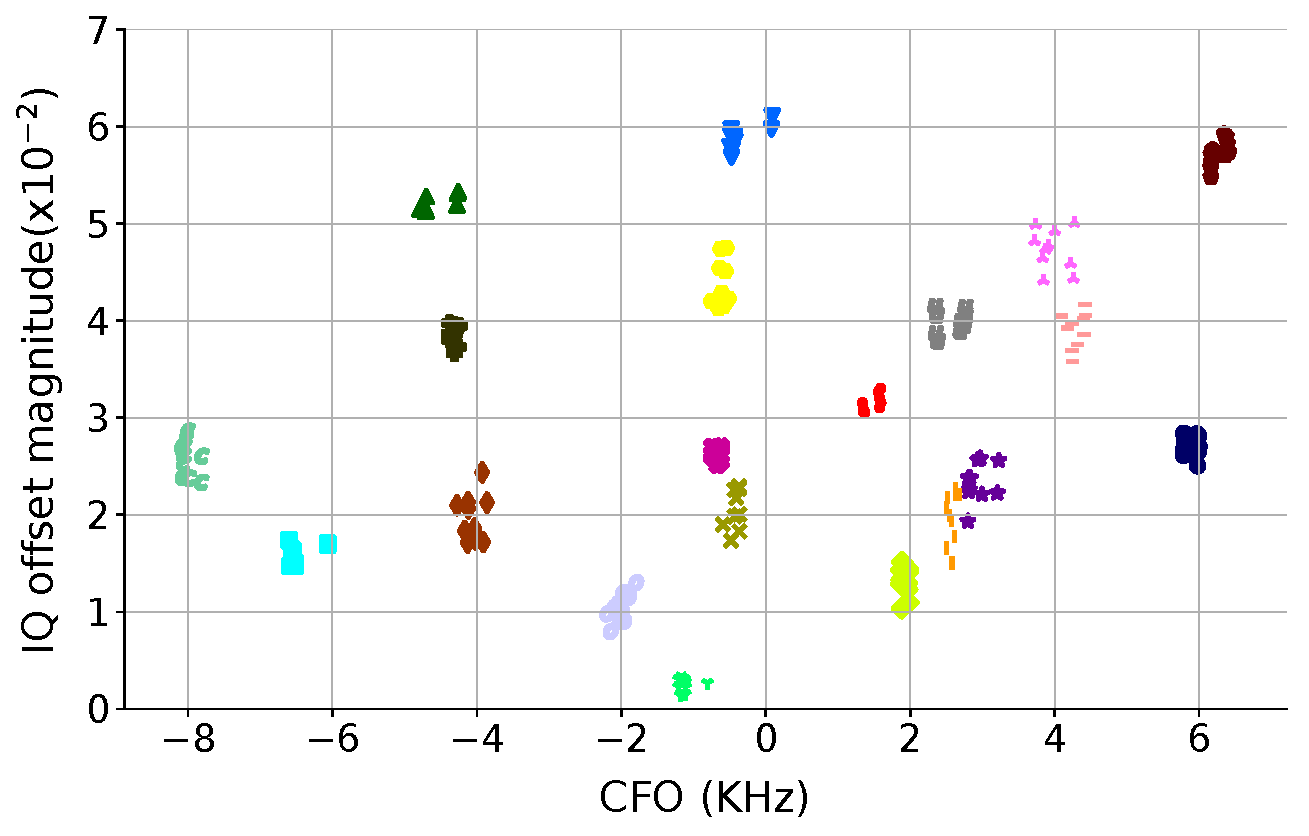
\includegraphics[width = \linewidth]{plots/ESP_CFOIQ.pdf} 
    \caption{CFO and IQ offset magnitude for 20 ESP32 chipsets}
    \label{fig:esp}
\end{figure}

\begin{figure}[t!]
    \centering
    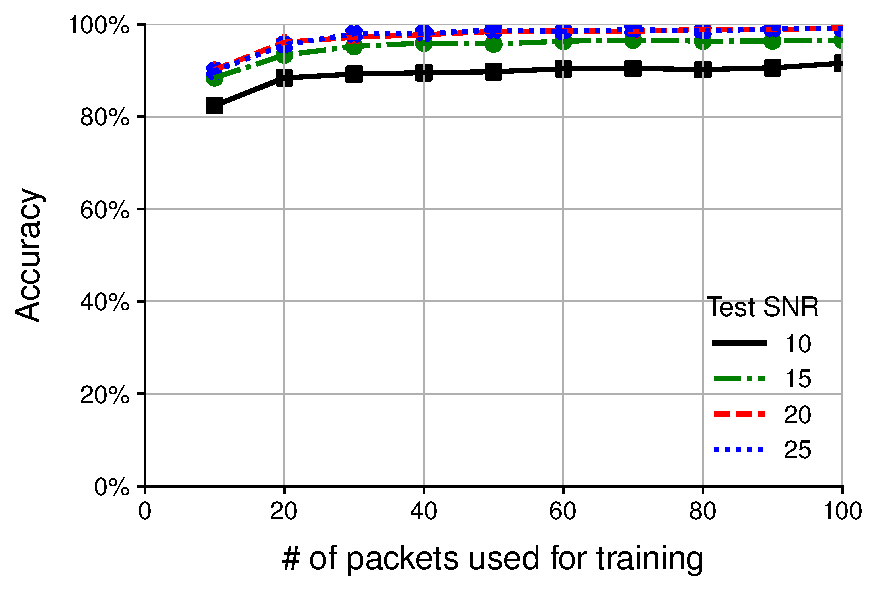
\includegraphics[width=\linewidth]{plots/accuracy_esp_train.pdf}
    \caption{Accuracy of classifying WiFi combo chipsets}
    \label{fig:esp_train}
\end{figure}

\begin{figure}[t!]
    \centering
    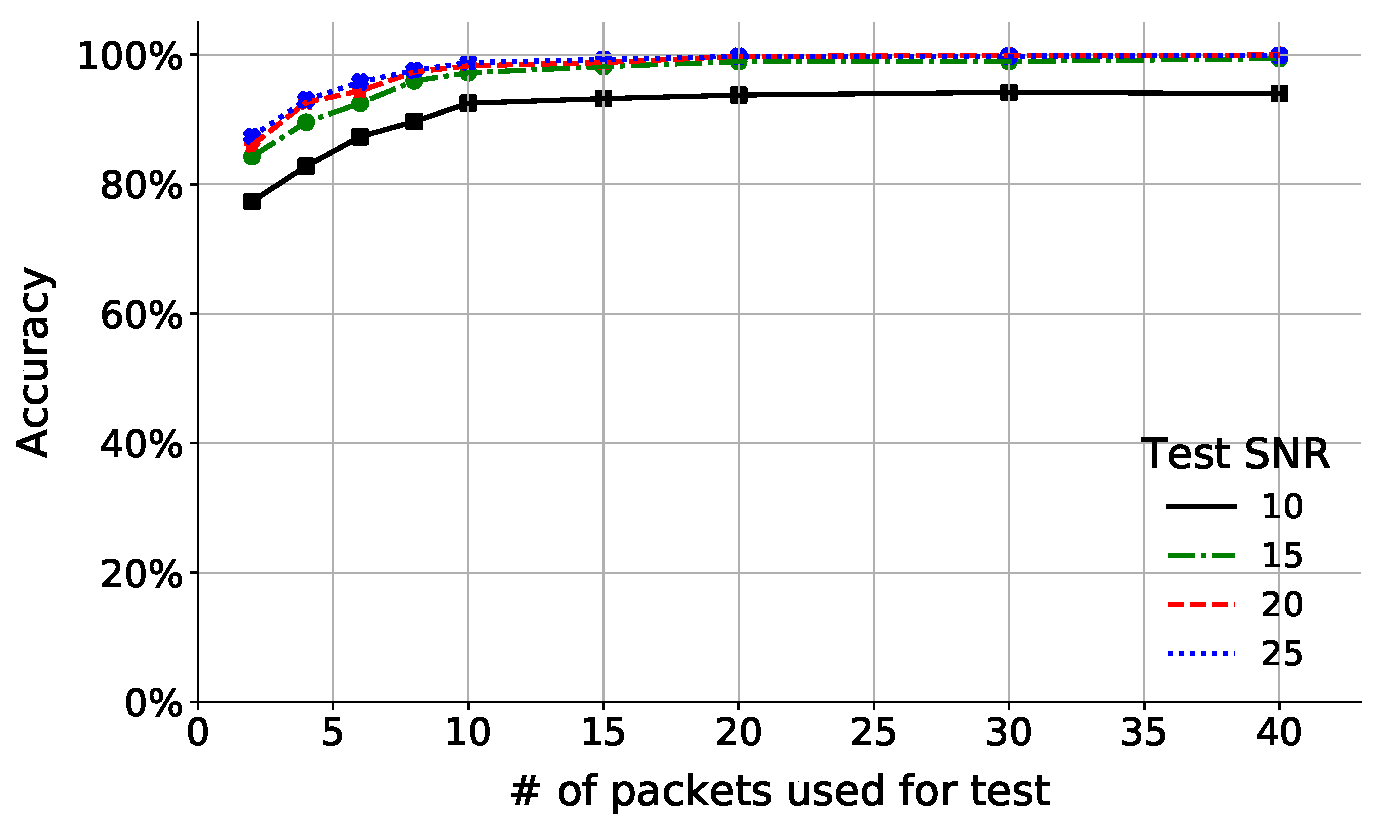
\includegraphics[width=\linewidth]{plots/accuracy_esp_test.pdf}
    \caption{Accuracy of classifying WiFi combo chipsets}
    \label{fig:esp_test}
\end{figure}

The first basic question to answer is how separable these chipsets are based on their RF fingerprints. Figure.~\ref{fig:esp} represents CFO and IQ offset (which are reported as the hardware imperfections which cause the most separabality in the literature) for 10 packets from each of these 20 devices. Although there exist a very few devices with close signatures, most devices look perfectly separable. Since all packets from the same device don't have the exact same CFO and IQ imperfection because of estimation error due to noise and tolerance of the hardware, the next question is how many packets we need to get from a device to build a robust and reliable profile for the device (fingerprinting stage), and having this profile for the device, how many packets we need to get from the device to be able to identify the device reliably in future (identification stage). 

Figure.~\ref{fig:esp_train} shows the test accuracy of classifying the devices compared to the number of packets used for training and building the profile of devices. For all SNR values, having 40 to 50 packets for training seems sufficient and there isn't much gain in accuracy after that. As mentioned earlier, most devices beacon more than this amount of BLE packets in a minute. Consequently, we need to isolate the device less than 1 minute to get enough packets to build a profile. 

Figure.~\ref{fig:esp_test} shows the test accuracy of classifying the devices compared to the number of packets used to decide on the classification for different test SNR values (the number of training packets is fixed to 50 per device). It is important to compare with the number of packets because obtaining more packets means that the target must be seen by the attacker for a longer period of time during the identification stage. For all SNR values, there isn't much accuracy gain when using more than 10 packets. In fact, although we can have more than 99 percent accuracy with having more packets during the training and test, having 50 packets during the training and 10 packets during the test is sufficient to get more than 98 percent accuracy for 15,20,25 dB SNR and more than 90 percent for 10 dB SNR.



\subsection{Identifiability in the wild}
\label{sec:results:field}

The question we intend to answer throught this section is \textit{Can we fingerprint the devices in field conditions? And are the device in-use such as phones, tablet, smart watches and so on distinguishable based on their RF fingerprints?}; Something that never has been addressed in prior RF fingerprinting work. 

To gain insights about the distinguishability of the devices in the wild, we collected BLE beacons from hundreds of devices in public areas such as five coffee shops and a library on January 2020. Even though we were analyzing captures from real-world devices, we were careful not to analyze the content of the packets we captured: we only analyzed the physical layer properties to perform our fingerprinting evaluation. %Moreover, we did not have any way of correlating a device's MAC address with the owner of the device and we only used these MAC addresses to compute a serial number in order to use as labels. 
One complication when running this uncontrolled experiment was that the MAC address of a device may change over due to MAC address randomization, causing the same device to be seen with more than one label. To mitigate this problem, for the data at a single location, we only consider devices that we have observed concurrently with other devices (assuming a single device can't have two MAC addresses at the same time). This will ensure that the MAC addresses that we considered are presenting different devices. This needs to be done only for the analysis in this section. For the evaluations presented in the next section, we did not need to filter out such MAC addresses.


\subsubsection*{Results}

From the last subsections, we know that we roughly need 50 packets from a device to build a robust profile for the target device. We use 50 packets for cross-validation and the rest of the packets to evaluate the accuracy. As mentioned in the last subsection, using 10 packets to decide about the identity of the device seems sufficient. Hence, we first average the features for 10 packets and then calculate the closeness or distance to targets' fingerprinting model. This results in having a set of devices $\{1,2,3,...,162\}$. 

The first question that needs to be answered is \textit{what is the chance that we confuse a device that is not our target with a device that we are looking for?}. To answer this question using our dataset, we take a device (MAC address) $i \in \{1,2,3,...,162\}$, build a profile for the $i$ device. Next, we calculate the false negative rate (FNR) using the rest of the packets from device $i$. Then, for each of the remaining devices, we use 10 packets and compute the features and compare with model of $i$ device. If it is identified as the device $i$, then it is considered as a false positive. The average of all these false positives is considered as the false positive rate (FPR) for device $i$. We compute the FPR for all $i \in \{1,2,3,...,162\}$ devices by repeating the same calculations.

Figure.~\ref{fig:fnr_cdf} demonstrates the CDF of FNR and Figure.~\ref{fig:fpr_cdf} demonstrates the CDF of FPR for these 162 devices. The average FNR is 2.53 percent and the FPR is 1.21 percent. Also the median FNR is 0 and the median FPR is 0.62 percent. Moreover, we see for more than 40 percent of the devices, there is no confusion (zero FPR) even in a dataset as large as 161 other devices. These devices are those that have a very unique and separable hardwaare imperfections (for instance, either a relatively large CFO or IQ offset or IQ imbalance). Having one of those perfectly identifiable devices can cause a serious privacy threat for the owner of the device. On the other hand, there are devices with commonly observed hardware imperfections (for instance, when both CFO and IQ offset are small). The FPR for these devices are even as high as 0.1. If the goal is identifying one of these devices in the field, we may quite often detect the device mistakenly when it is not present.

\begin{figure}[t!]
    \centering
    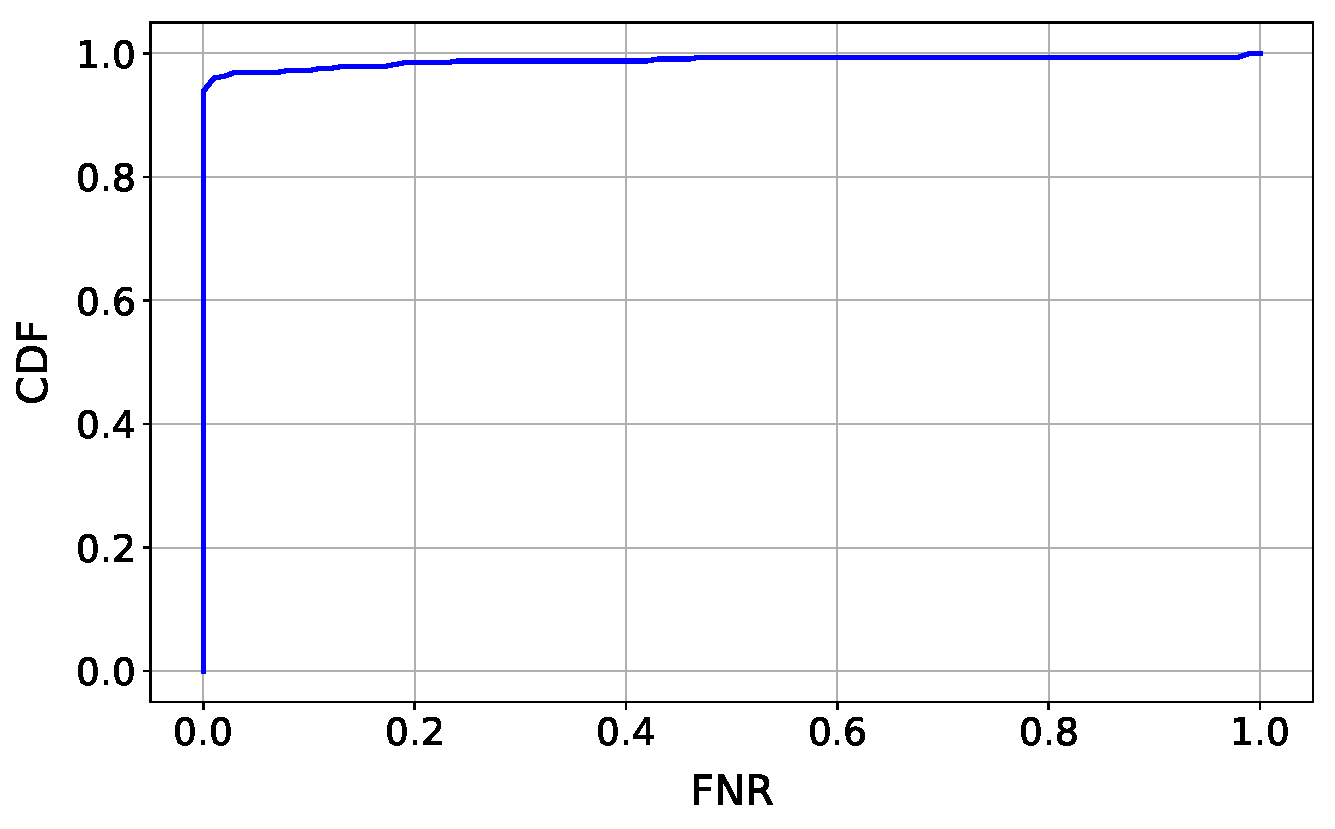
\includegraphics[width = \linewidth]{plots/fnr_cdf.pdf} 
    \caption{CDF of FNR for the devices in the wild. Average FNR = 2.53\%. Median FNR = 0\%.}
    \label{fig:fnr_cdf}
\end{figure}

\begin{figure}[t!]
    \centering
    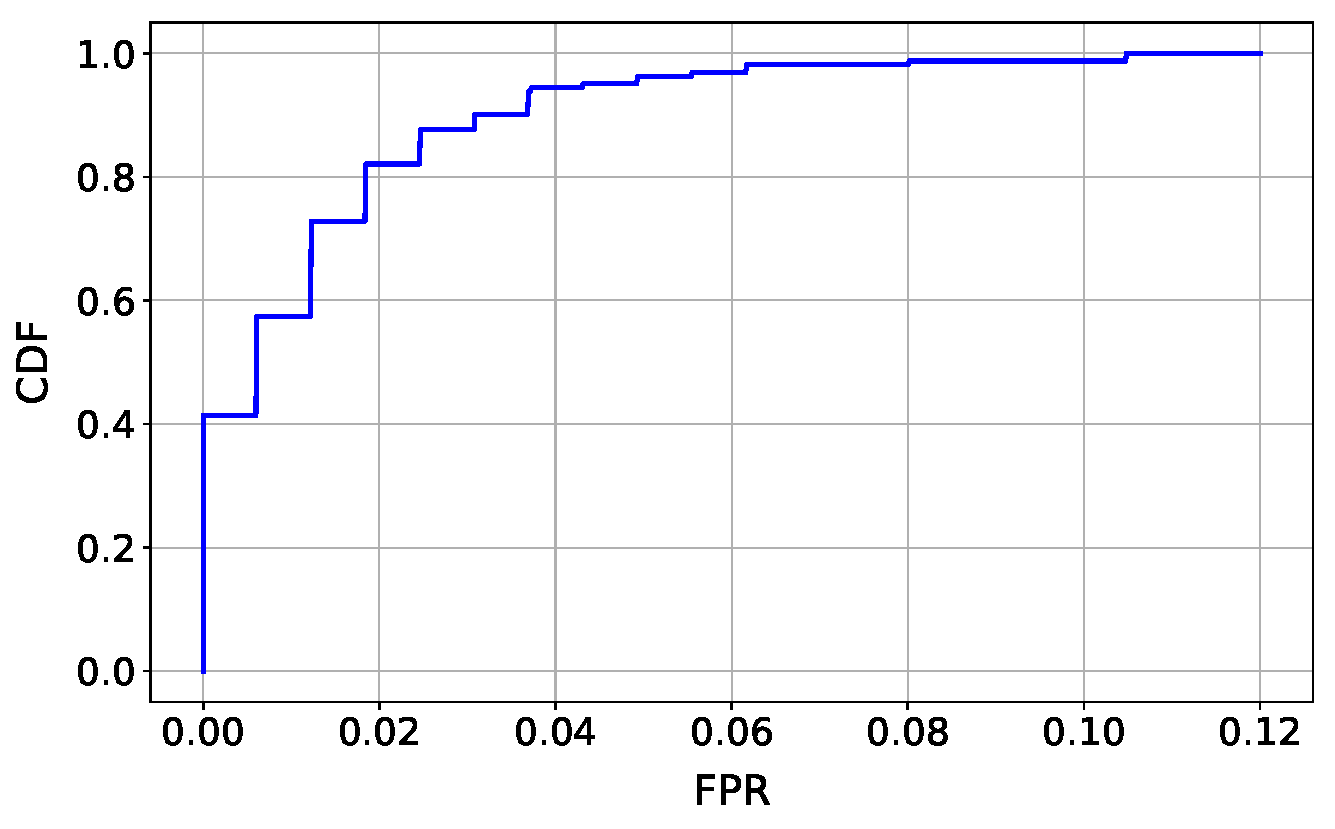
\includegraphics[width = \linewidth]{plots/fpr_cdf.pdf} 
    \caption{CDF of FPR for the devices in the wild. Average FPR = 1.21\%. Median FPR = 0.62\%}
    \label{fig:fpr_cdf}
\end{figure}

The next question to answer is \textit{what are these devices that we confuse? Are we mostly confusing the devices from the same model?} We used the technique proposed in~\cite{celosia2020close} to distinguish the Apple products from others. About 76 percent (123 devices) of the dataset are Apple products which is the dominant majority of the observed devices. This is mainly because of continuity protocol and Find My feature in Apple products which make them constantly beacon BLE packets. This dataset was collected before COVID19. These days, while Apple product are still the majority of beaconers, we expect to see a much greater share of other devices (e.g. Android phones) as many contact tracing apps make the phones beacon BLE signals. 

We repeat the same experiment as above, however, this time we break up the results based on whether the device is an Apple product or not in Table~\ref{tab:apple_table}. The FPR between Apple devices (first row) is greater than the average FPR we reported before and the FPR between Apple product and the devices that are not Apple products is very small (third row). The reason could be that as one might expect, the hardware imperfections of the devices from the same make are more likely to be close too each other than the devices with different make and model. In fact, the lab experiments in Section~\ref{sec:similarity} also verifies that the hardware imperfection distributions of devices from the same make and model could be different. Consequently, distinguishing devices from different models should be easier on average.

% \begin{table}[]
%     \begin{tabular}{|l|l|}
%     \hline
%      Device type&FPR \\ \hline
%      &  \\ \hline
%      &  \\ \hline
%      & \\ \hline
%     \end{tabular}
% \end{table}

\begin{table}[]
    \centering
    \begin{tabular}{|l|l|l|}
    \hline
    Devices Considered&FPR (percent)&FNR (percent)\\ \hline
    Apple Products& \quad \quad 1.91& \quad \quad 2.40\\ \hline
    Not Apple Product& \quad \quad 1.15& \quad \quad 2.94\\ \hline
    Apple vs Not Apple& \quad \quad 0.15& \quad \quad \quad - \\ \hline
    \textbf{All Devices}& \quad \quad \textbf{1.21}& \quad \quad \textbf{2.53}\\ \hline
    \end{tabular}
    \caption{FPR and FNR comparison for Apple products and other devices.}
    \label{tab:apple_table}
\end{table}

The third question to answer is that \textit{which one of these hardware imperfections contribute the most in distinguishing these devices?} Table~\ref{tab:ablation} shows the FPR and FNR when using CFO, IQ offset and IQ imbalance separately and together by repeating the same experiment as before. CFO contributes the most as it can have a wider range of values for different devices compared to IQ imperfections. However, CFO is not sufficient to get the best result. IQ imperfections resolve the confusion in some cases in which the two device have similar CFO values and reduce thee FPR from 2.42 percent to 1.21 percent. This also can be observed in our controlled lab experiments in Figure~\ref{fig:cfoiq} where some devices have CFO values close to each other but their difference in IQ imperfection helps us with distinguishing those devices. Furthermore, as we will see in Section~\ref{sec:temp}, temperature can significantly affect CFO while it does not have any notable impact on IQ imperfections. As a result, IQ imperfections can come to the rescue in situations in which the target might experience temperature changes. Moreover, the FPR and FNR when only using CFO computed by our method, is better than FPR and FNR when use the baseline CFO computed by existing techniques described before. This significantly impacts the identification when we aim at identifying a device in the presence of a large set of other devices. In fact, as discussed in Secion~\ref{sec:similarity} having a method to measure hardware imperfections with fine-granularity is necessary to RF fingerprinting; otherwise the device with close fingerprints will be easily confused.


\begin{table}[]
    \centering
    \begin{tabular}{|l|l|l|}
    \hline
    Features used&FPR (percent)&FNR (percent)\\ \hline
    Baseline CFO& \quad \quad 7.41& \quad \quad 3.49\\ \hline
    CFO only& \quad \quad 2.42& \quad \quad 2.45\\ \hline
    IQ offset only& \quad \quad 19.84& \quad \quad 2.39\\ \hline
    IQ imbalance only& \quad \quad 32.53& \quad \quad  1.52\\ \hline
    \textbf{All Features}& \quad \quad \textbf{1.21}& \quad \quad \textbf{2.53}\\ \hline
    \end{tabular}
    \caption{Seperability of each feature alone. CFO contributes the most but IQ imperfections could further improve the identification.}
    \label{tab:ablation}
\end{table}

\subsection{Identifying the targets}
\label{sec:results:case1}
Throughout the evaluation section, so far we have observed that there is a high chance that we can properly identify the devices in-use in the field. In this section, we conduct an experiment to demonstrate one of the scenarios that this attack might be deployed. We have 17 targets outside of the set of devices collected in the wild. These targets are listed in Table~\ref{tab:targets} that we want to identify. Each target is isolated for a while to get at least 50 packets for training and 50 packets for the evaluation set. These targets are profiled using the training and evaluation data and the profile of each device is stored and used in the rest of the study to compute FNR and FPR. 

Between 2-7 days later, we took these targets to a food court and turn on your sniffer there. This data is used to compute the FNR for these 17 targets using the stored profile for each of the targets. We also use the captures from the aforementioned coffee shop data (this time we don't filter out any MAC address and we consider all MAC addresses even with a very small number of packets) in which none of the targets are present, to compute the FPR for these targets. The way that FNR and FPR are calculated is that, in each 10 seconds of the captures, we see if there is any MAC address (at least one MAC address) whose hardware imperfections matches the stored profile of a specific target. If there exist such MAC address, then we have identified that specific target device in that second. Then FNR and FPR are computed depending on whether that target was actually present there or not. In fact FNR here is the percentage of time a specific target device is there but we think it's not, and FPR is the percentage of time that a specific target device is not present but we think it is. 

\begin{table}[]
    \centering
    \begin{tabular}{|l|l|l|}
    \hline
    Label: Device&Label: Device&Label: Device\\ \hline
    1: iPhone 10&7: iPhone 10&13: MacBook Pro\\ \hline
    2: iPhone 8&8: iWatch&14: Thinkpad\\ \hline
    3: iPhone 11&9: iPhone 10&15: AirPod\\ \hline
    4: Bose Headset&10: iPhone 8&16: Pixel 2\\ \hline
    5: iWatch&11: iPhone 10&17: Pixel 5\\ \hline
    6: iPhone 8&12: iWatch& \\ \hline
    \end{tabular}
    \caption{17 target devices used for this experiment and their label numbers that are used in other figures}
    \label{tab:targets}
\end{table}

\subsubsection*{Results}
Figure~\ref{fig:fpr_fnr} presents FNR-FPR for these 17 targets. The average FNR of these targets is 3.21 percent and the average FPR is 3.5 percent. As shown in the figure, although there are a few devices with high FNR and FPR, most devices have distinguishable and persistent hardware imperfections, resulting in low FNR and FPR. If an individual owns one of these well-identifiable device, then they could be in a serious threat of being identified by the attackers at their desired location. 

Figure~\ref{fig:fpr_time} demonstrates the false positive occurrences for all of our targets in the longest coffee shop capture. Each time there is a bump, it means that at least one device was detected as the corresponding target falsely. As we observe, most of the false positives continue for a while, possibly because a device with a similar hardware imperfections as the target entered the coffee shop and left after a while. 
%In some cases, a MAC address is falsely detected as our target but after a while it dissapears and a new MAC address causes the false positive occurance, possibly because the device has changed its MAC address and the new confused MAC address is the same device that was confused before which has changed its MAC address. 
There also exists a very few false positive occurrences that last for a few seconds. This is because sometimes we did not get enough packets from a device in 10 seconds and the hardware imperfections of the very few noisy packets looked like our target. However, after getting more packets from that device, it turns out we were wrong and false positive is resolved in the next time slots. Finally, its worth mentioning that on average, we saw 18 unique MAC addresses in each 10 seconds and overall we saw 259 unique MAC addresses during this 48 minute capture at a coffee shop.

\begin{figure}[t!]
    \centering
    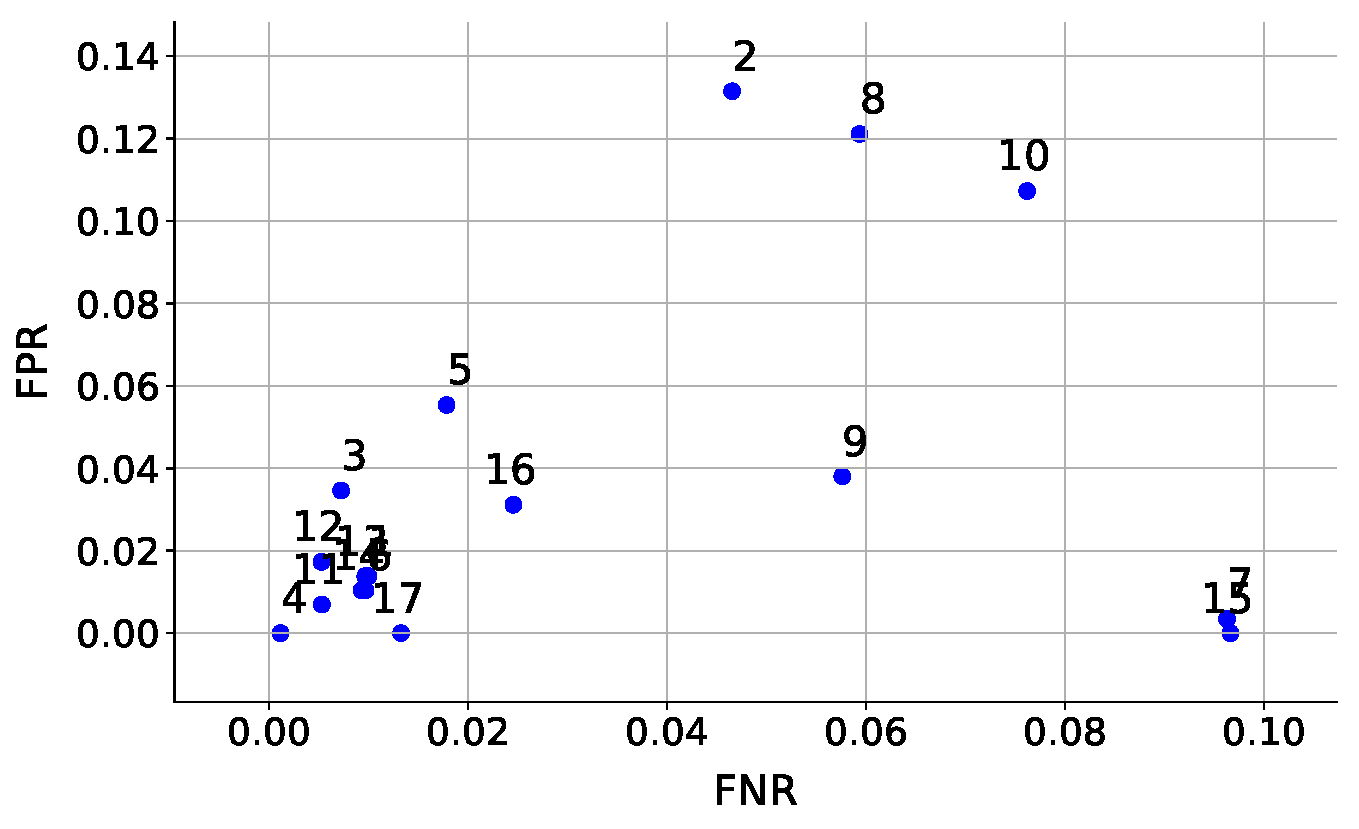
\includegraphics[width = \linewidth]{plots/fpr_fnr_10sec.pdf} 
    \caption{FNR-FPR for 17 targets. Label numbers are assigned in Table~\ref{tab:targets}.}
    \label{fig:fpr_fnr}
\end{figure}

\begin{figure}[t!]
    \centering
    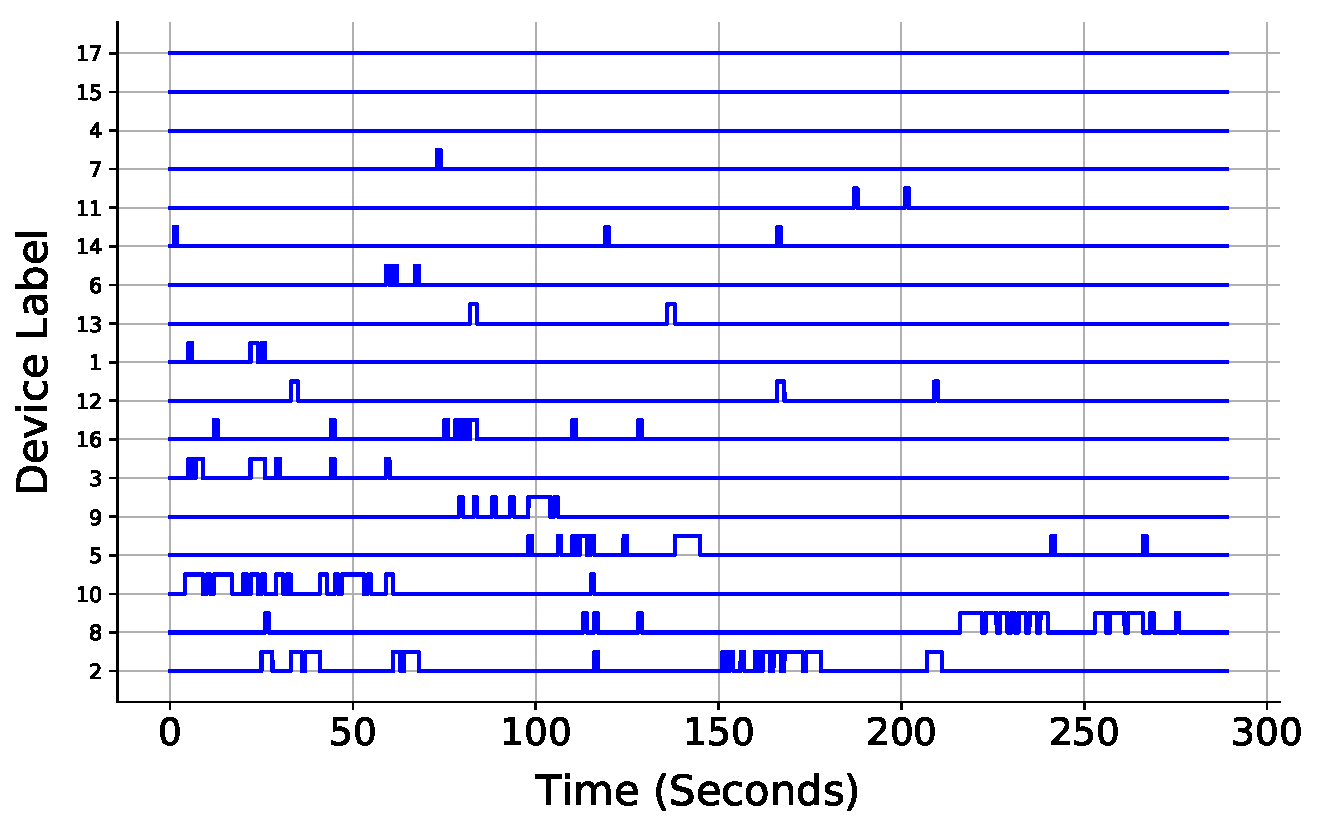
\includegraphics[width = \linewidth]{plots/fpr_time_10sec_sort.pdf} 
    \caption{Each line represents FPR occurances over time for one of the 17 targets. Label numbers are assigned in Table~\ref{tab:targets}.}
    \label{fig:fpr_time}
\end{figure}










\subsection{Case Study : Tracking a person}
\label{sec:results:case2}

\begin{figure}[t!]
    \centering
    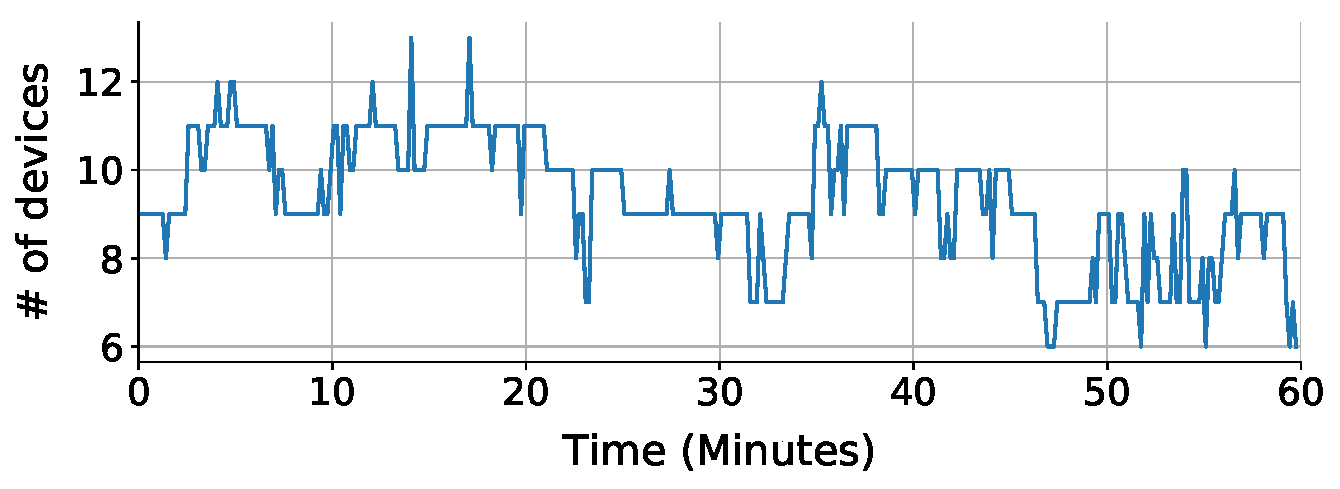
\includegraphics[width = \linewidth]{plots/case_study_iphone_devno.pdf} 
    \caption{Number of unique MAC addresses observed over time duuring the experiment of tracking iPhone}
    \label{fig:iphone_no}
\end{figure}


\begin{figure}[t!]
    \centering
    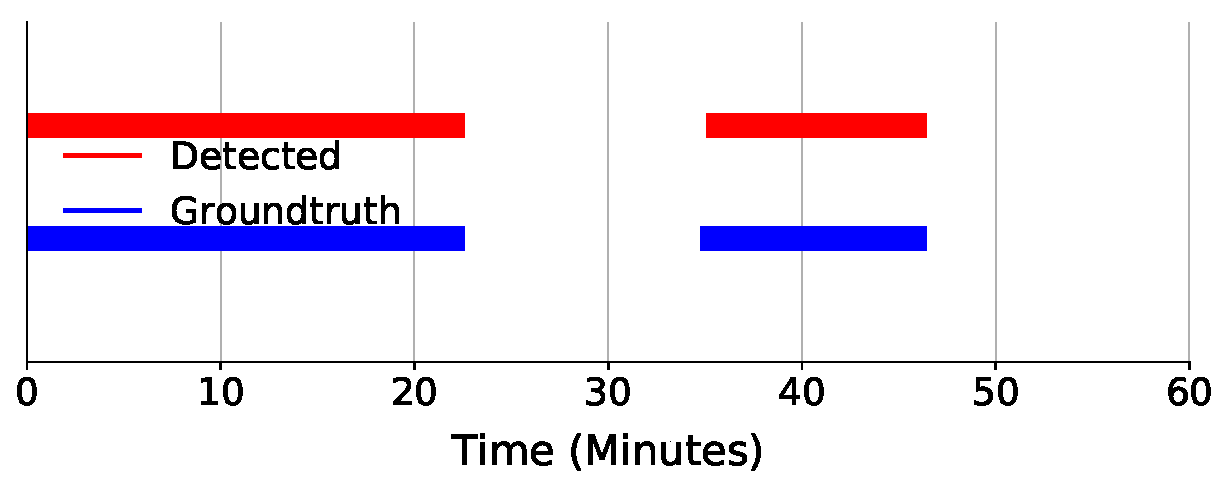
\includegraphics[width = \linewidth]{plots/case_study_iphone.pdf} 
    \caption{The blue bar represents the time that the iPhone target was present and the red bar represents the time that our algorithm detected the presence of the iPhone}
    \label{fig:iphone}
\end{figure}


\begin{figure}[t!]
    \centering
    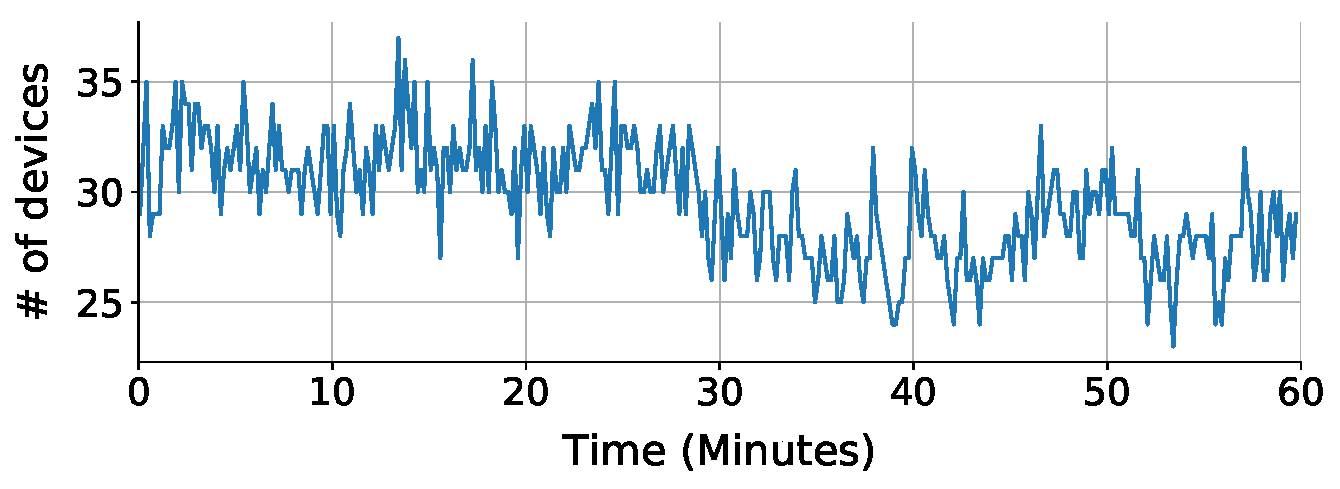
\includegraphics[width = \linewidth]{plots/case_study_android_devno.pdf} 
    \caption{Number of unique MAC addresses observed over time duuring the experiment of tracking Pixel 5}
    \label{fig:android_no}
\end{figure}

\begin{figure}[t!]
    \centering
    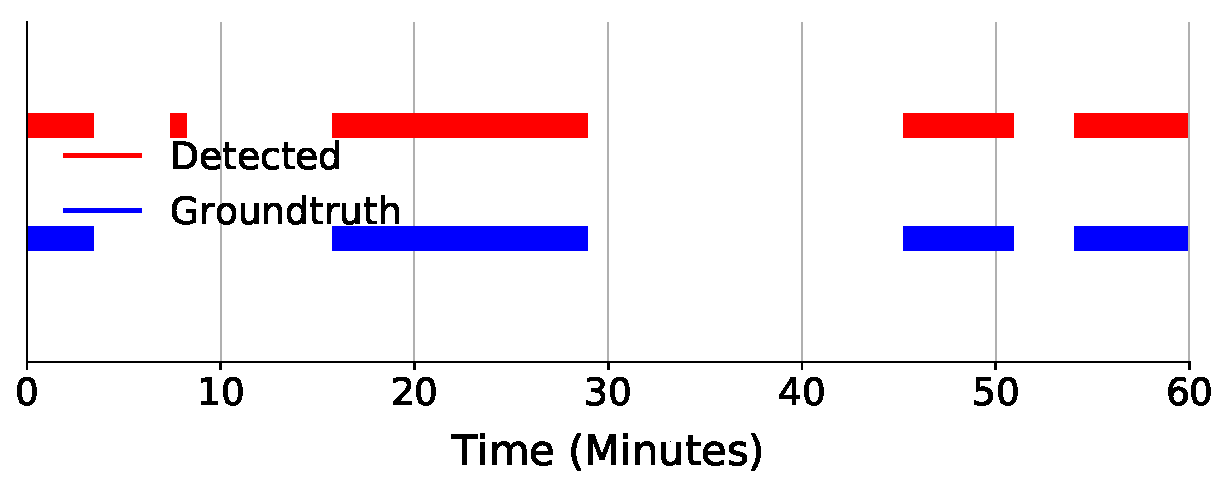
\includegraphics[width = \linewidth]{plots/case_study_android.pdf} 
    \caption{The blue bar represents the time that the Pixel 5 target was present and the red bar represents the time that our algorithm detected the presence of the Pixel 5}
    \label{fig:android}
\end{figure}

In this section, we deploy and evaluate a typical scenario that our RF fingerprinting attack might take place. We isolate an iPhone device that belongs to a volunteer, to profile the device (fingerprinting stage). 2 days later, we put our sniffer close to their house. The goal is to detect the presence of the person whenever they come home (Identification stage). We track their presence for one hour during which the person walks inside and outside the house 2 times. Figure~\ref{fig:iphone_no} shows the number of unique MAC addresses observed during this time. As we count the number of MAC addresses in a short duration of every 10 seconds, this also represents the number of devices observed over time. 

The blue bar shown in Figure~\ref{fig:iphone} demonstrates the periods of time at which the person was inside the house and the signal of their phone was stronger than the power level threshold set by the sniffer. The red bar in the same plot shows the time durations which [name] thinks the person was present. They perfectly match except for the beginning 10 second of the second entrance of the person which we miss because we were not able to receive enough packets from their phone (in each 10 seconds, if we don't receive the 10 packet we need from a MAC address, we look back at previous time slots and use the packets we received from that MAC address previously). 

Next, we repeat the same experiment when the volunteer is carrying a pixel 5 phone. This time, we also reduce the power level threshold that our sniffer captures the signals. As shown in Figure~\ref{fig:android_no}, we capture signals from more devices in a wider range from the sniffer. Figure~\ref{fig:android} shows the groundtruth time when the person was present and the time which [name] detected the presence of the person. This time, we mistakenly think our target was present for about 50 seconds while they were not. This confusion happened for a single MAC address and was resolved when the MAC address disappeared. As we have increased the range that our receiver can receive, this device most likely belonged to a person passing by around the house. In both scenarios, we demonstrated that one can deploy our RF fingerprinting attack in a real-world scenario with high accuracy, threatening the owner of the device.


\subsection{Temperature effect on identifiability}
\label{sec:temp}

\begin{figure}[t!]
    \centering
    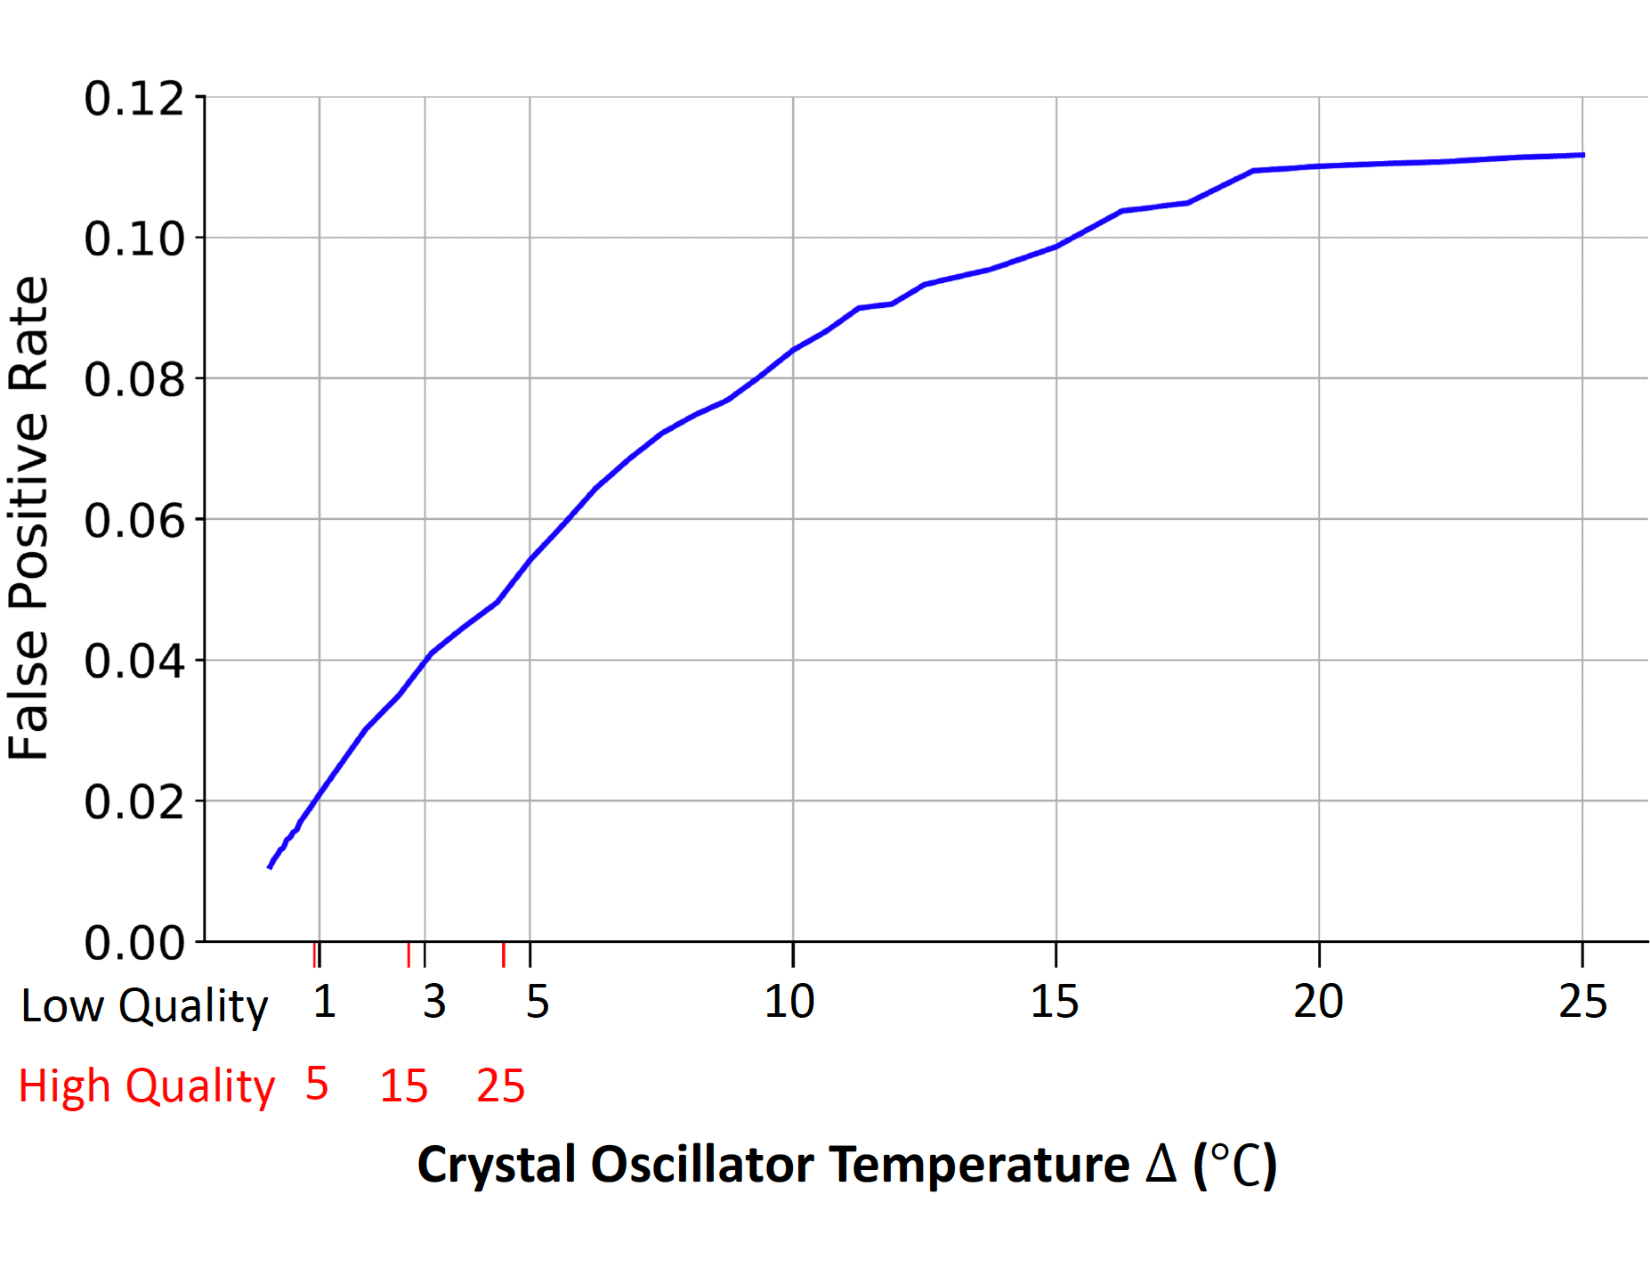
\includegraphics[width = \linewidth]{plots/fpr_temp.pdf} 
    \caption{ }
    \label{fig:fpr_temp}
\end{figure}

As mentioned earlier, most devices that beacon BLE packets, randomize their MAC address about every 15 minutes. Consequently, as the only way to label the devices in the wild is their MAC address, we at most have 15 minutes of data with the same label for most devices in the field. Although during this 15 minutes, the temperature of some of these devices may change due to the change in activity level on the device (such as calling or opening apps on the phone), most devices will maintaing roughly the same temperature. Consequently, the effect of temperature on the ability to identify the devices is not well-represented in the field data. In this section, we ask \textit{what would be the effect of temperature changes on the ability to identify the devices in the field?}

According to Section~\ref{sec:similarity}, temperature changes can significantly affect CFO of the device even upto several KiloHertz, while it does not affect IQ imperfections noticeably. The impact of temperature on frequency drift has been evaluated in many documents. For instance, ~\cite{temp_cfo1} demonstrates the Bechmann curve (frequency drift versus temperature) for an AT-cut crystal for different crystal cutting accuracies. Generally speaking, three observations can be made from this curve. First, the frequency drift (which results in changing CFO) increases as the temperature changes more and more. Second, in the temperature interval that personal electronic devices may experience, frequency drift is linearly dependent on the temperature changes. Third, crystals with different cutting accuracies experience different amount of frequency drift for the same amount of change in temperature.

When the device temperature changes, the CFO of the device changes and the device will have a different CFO compared to when it was fingerprinted. Consequently, the device will not be identifiable resulting in false negative. To mitigate this, we should extend the CFO values that is expected to be received from the target device. For instance, assume  $\Delta T  ^\circ C$ temperature change causes $\Delta f$ KHz change in CFO. Assume a device was fingeprinted in $T_0 ^\circ C$ and the CFO was recorded as $f_0$ KHz. In order to make sure (ignoring other factors that may affect RF fingerprints) that our identification system can tolerate upto $\Delta T ^\circ C$ temperature change and we will identify the device if its temperature is anywhere between  $[T_0-\Delta T, T_0+\Delta T]$, we must accept that any CFO value between $[f_0-\Delta f, f_0+\Delta f]$ KHz matches the CFO of our device. The consequence of extending the acceptable boundaries of CFO is that other devices with CFO in this range might be mistakenly identified as our target (if their IQ imperfections are also close to each other). This will increase the false positive rate (FPR) of our identification system. In fact, as $\Delta T$ increases, it will cause more change in CFO which forces us to extend the CFO boundaries in order to maintain the same false negative rate (FNR). By extending the CFO boundaries, there will be more and more devices out in the field that are not our target but their CFO fall inside the accepted CFO boundary of our target, resulting in higher FPR.

Now we use our field data to analyze the effect of temperature change on identifying the device. We follow the same approach as described in Section~\ref{sec:results:field}. The difference is that this time we use the analysis discussed above to set the threshold or boundaries for the target. For any temperature change of $\Delta T  ^\circ C$, we use the cruves in~\cite{temp_cfo1} to find the corresponding change in CFO $\Delta f$. We set the threshold for CFO equal to $\Delta f$ so that we make sure our identification system can identify the target if the temperature changes upto $\Delta T  ^\circ C$. For other imperfections (IQ offset and imbalance), we chose the threshold the same way as before as they are not noticeably affected by temperature according to our controlled lab experiments. Figure~\ref{fig:fpr_temp} represents FPR for different values of $\Delta T$ for two crystal with different cutting accuracies. As mentioned earlier, temperature change causes less change in CFO for high quality crystals with high cutting accuracy compared to low quality crystals with low cutting accuracies. As a result, if we assume the device is using a high quality crystal, the FPR will increase less as we don't need to push CFO boundaries too much to handle possible changes in temperature. Figure~\ref{fig:fpr_temp} demonstrates this fact assuming a very high quality crystal with 0 minute cutting accuracy is used as well as what would happen if a very low quality crystal with 8 minute cutting accuracy is used. 

According to Figure~\ref{fig:fpr_temp}, the temperature can potentially increase FPR for a fixed FNR rapidly for low quality crystals and make the identification less accurate. This can affect the ability of attacker in some scenarios if the victims use their personal electronic devices to run heavy apps quite often or if the device was fingerprinted when its temperature was not in a normal temperature such as the room temperature. Furthermore, not that for low quality crystals, when the change in temperature is too much, CFO almost does not help in identification as we had to push the CFO boundaries to include almost all possible CFO values seen for the devices in the field. Consequently, the FPR is the same as if we only use IQ offset and IQ imbalance.








%!TEX root = paper.tex

\section{BLE Fingerprinting Toolkit}
\label{sec:methodology}

In this section, we develop a systematic toolkit to extract fingerprints of the BLE wireless transceivers in the
portable electronic devices like smart phone and smartwatches. First, we explore and understand ways to fingerprint the wireless transceivers. Next, we develop a 
methodology which can be used to extract the hardware imperfection information from the BLE tranmissions, wherein, 
we develop a joint estimation technique to extract the identifying information accurately. 

\subsection{BLE is difficult to fingerprint} %{{{
\label{sec:motivation:diff}

Although BLE poses a new and significant threat to the location privacy of
mobile device users, the protocol's design makes it extremely difficult to
obtain a reliable fingerprint of a device.
%
Specifically, the BLE protocol includes built-in mechanisms to prevent MAC
address fingerprinting, and the physical-layer signal is so simple that it is
difficult to produce a unique and fine-grained fingerprint.

\vspace{0.5em}
\noindent\textbf{MAC-Layer Fingerprinting:} 
%
At its most basic level, BLE's design frustrates MAC-layer fingerprinting.
%
Although BLE advertisements contain a full 6-byte MAC address that is unique to the
advertising device, the BLE protocol also has built-in cryptographic MAC randomization.
%
Fortunately, prior work found (and we confirmed) that mobile devices are
properly implementing BLE's MAC address randomization~\cite{Iphonetracking_becker,MACRandomizationfail_Martin}.
%
Namely, they found devices are following the BLE specification and periodically
(every 10--15 minutes) randomizing their MAC addresses~\cite{BTsigprivacy}.
%
However, this work also found that an attacker persistently following the target
device can track a device across MAC address changes by observing other fields
in the BLE beacon packet that were not reset properly after the MAC was
randomized.
%
This attack is extremely limited, as it requires an attacker to
persistently follow a target to track it; therefore, if the attacker misses a
MAC randomization cycle it can no longer identify the target.

\begin{figure}
    \centering
    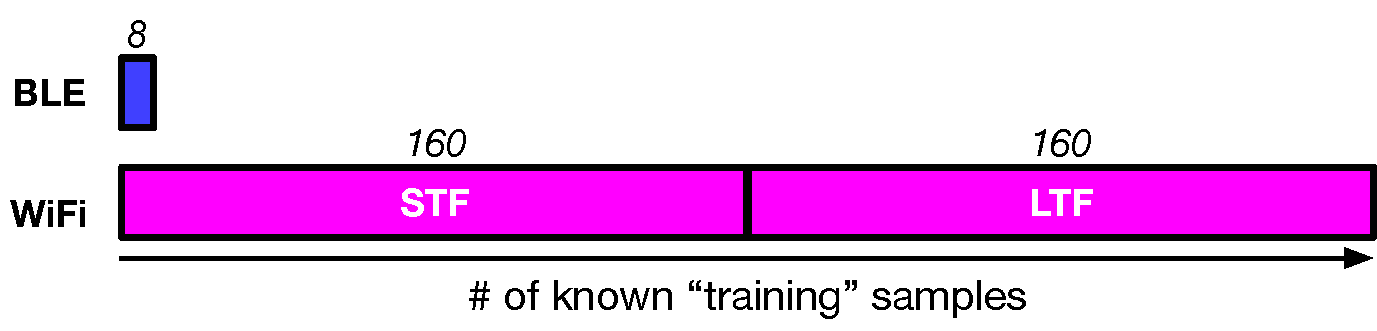
\includegraphics[width=\linewidth]{plots/knownsamples}
    \caption{
      BLE packets have very few known samples for physical layer fingerprinting.
    \label{fig:2}
  }
\end{figure}



\vspace{0.5em} \noindent\textbf{Physical-layer fingerprinting:}
Therefore, one cannot use MAC layer fingerprinting for BLE transmissions.
%
Physical layer fingerprinting is possible due to each radio having unique
hardware imperfections in its transmitter chain.
%
Several hardware imperfections have been explored for RF fingerprinting in the literature. 
For instance, transient portion of the signal has been proposed as a unique signature to 
classify different wireless devices~\cite{extraction_rehman, transientID_danev}, even Bluetooth
signals~\cite{transientBT_Hall}. However, the transient portion of BLE and Bluetooth signals
is only about 2 microseconds and contains insufficient information to uniquely identify 
a device among tens of devices. Modulation-shape features have also been explored for RF
fingerprinting devices such as RFID transponders~\cite{rfidphysical_danev}. However, 
the Gaussian shape in GFSK modulation of BLE signals is generated digitally in most 
personal electronic devices such as phones, and thus, cannot be used as a unique fingerprint.
In the WiFi literature, CFO and IQ imperfections (IQ origin offset and IQ imbalance) are 
two well recongized features which have been shown to be the most separable features for 
RF fingerprinting~\cite{Brik_radiometric}. However, can we extract the CFO and IQ imperfection signatures from the
BLE signals to uniquely fingerprint the devices?
% Now the question is: Do these hadrware imperfections (CFO and IQ imperfection) that have 
% been demonstrated to be the most effective in RF fingerprinting, exist in BLE signals as well?
%Interestingly enough, even though BLE signals are much less complex than WiFi, many mobile devices introduce the  same complex hardware imperfections in BLE as they do in WiFi. This is 
%\todo{talk suitability and other features}

Extracting the CFO, IQ offset and imbalance is often challenging for the BLE signals.  
%
Primarily, as the design of BLE's physical layer is so simple that it is unlikely to
estimate the CFO and IQ imperfections precisely.
%
%The reason is, BLE is an extremely low-energy protocol: BLE's physical-layer signal is designed to require simple hardware to transmit and receive messages.
% 
BLE signals are generated by representing the transmission bits as basic 
Gaussian Frequency Shift Keying (GFSK) modulation. Often the CFO and IQ impairments 
are embedded in the BLE signals as a part of transmitting them from the radio.
Ideally, an attacker would need to receive these samples, and extract these impariment 
from the simple GFSK signal. The standard BLE receivers can decode the 
packet without explicity correcting for CFO or IQ imperfections. There are two key challenges 
with extracting these impairments:

First, since the BLE signals are simple narrowband FSK signals with no special mechanism to extract
the CFO and IQ imperfections makes it challenging. For example, the WiFi signals are wide-band signals
whose decoding algorithms are complex and correct for CFO and IQ imperfections to achieve accurate decoding.
In constrast, BLE signals use FSK modulation, where in the receiver uses the preamble to identify the mid-point
of the two frequency used for data modulation, and uses that as a calibration point, to decode bits as 1 or 0. 
Furthermore, the narrowband of 1 MHz signal is no help. For example, WiFi signal has a bandwidth of 20 MHz, wherein, 
the phase change over the 20 MHz wave is used to measure the carrier frequency offset, therefore provding a much more accurate measurement. For example, even xx KHz offset would cause a phase change of yy degree in xx usec. In contrast, the bandwidth of BLE of 1 MHz would require zz usec of data to measure the same offset.  

\if 0
%
Such a simple transmitter will not have the complex hardware
impairments that have made it possible to fingerprint other mobile device protocols, 
namely WiFi~\cite{vohuuusrp,Brik_radiometric,deviceID_kose}.
%
% Since these imperfections are
%caused by manufacturing variability, they can even produce a fingerprint for
%devices from the same make and model.
%
%
%of a particular mobile
%device's radio is comparing known patterns in a signal received from that
%transmitter to the imperfect signal received from the transmitter.
%
\fi

Second, BLE transmissions do not require a significant number of known ``training''
samples for a receiver to use to correct for imperfections before decoding.
%  
These limitations make it difficult to apply existing physical-layer techniques~\cite{vohuuusrp,Brik_radiometric,deviceID_kose,Intrusion_hall,suskitransient,deeplearning_merchant,lora_robyns,gopalakrishnan2019robust}
to fingerprint BLE.
%
The problem is, these techniques have been developed for protocols, such as
WiFi, that require extremely accurate
corrections of impairments before they can even be decoded.
%
Figure~\ref{fig:2} shows a comparison of the length of a typical
BLE beacon packet compared to a typical WiFi packet.
%
BLE packets only include 8 known samples, whereas WiFi packets include 
a total of 320 known samples. Furthermore, the preamble or training sequence 
for WiFi is designed to estimate the CFO and IQ impairments accurately to decode
the data. 



% \subsection{BLE is ubiquitous }

% Our goal is to identify the wireless transceiver, which could leak the location and be able to identify them. Most
% transcevivers today use MAC address randomization to enable to privacy. Hence, we focus on building a methodlogy to
% extract the physical tranceivers fingerprints to identify the emission and thereof their proximity.

% A natural way to perform finger-printing would be to leverage WiFi signals; as there has been extensive literature on extracting the WiFi fingerprinting. However, suprisingly the WiFi transceiver are quiet i.e. they only transmit when the user uses the portable devices, and performs in-frequent beacons. Furthermore, WiFi transceivers are long-range making it hard to find proximity of the user. Finally, some of the portable devices do not have WiFi transceivers. Thus using WiFi wouldn't scale as an attack.

% On the otherhand, bluetooth low energy (BLE) tranceviers are part and parcel of all portable devices. Next, the BLE emissions are short range making them vulunerable in providing the proximity of the user. Finally, the BLE was designed for advertisement i.e. they beacon frequently and futhermore, many devices use BLE for continuity protocol
% \todo{descirbe the protocol}. In summary, BLE emissions are all ubiquitious, pervasive and beaconing frequently. However, the BLE protocol randomizes the MAC address every 15 minute to provide privacy to the user. However, they are still vulnerable to the physical layer fingerprinting. 


\subsection{Novel Technique to Extract the RF fingerprints using the BLE}

We present a new physical layer fingerprinting technique that
can uniquely identify BLE devices.
%
We first describe why surprisingly, even though BLE signals are much less
complex than WiFi, many mobile devices introduce the  same complex hardware
imperfections in BLE as they do in WiFi.
%
Then we present a new algorithm to robustly and accurately extract these
WiFi-like imperfections from BLE packets.
%
The key contribution of our algorithm is overcoming the primary limitation of
BLE physical layer fingerprinting: its short known samples in its preamble
(Section~\ref{sec:motivation:diff}).

\subsection{BLE has WiFi-like signal imperfections} %{{{

\begin{figure}[t!]
    \centering
    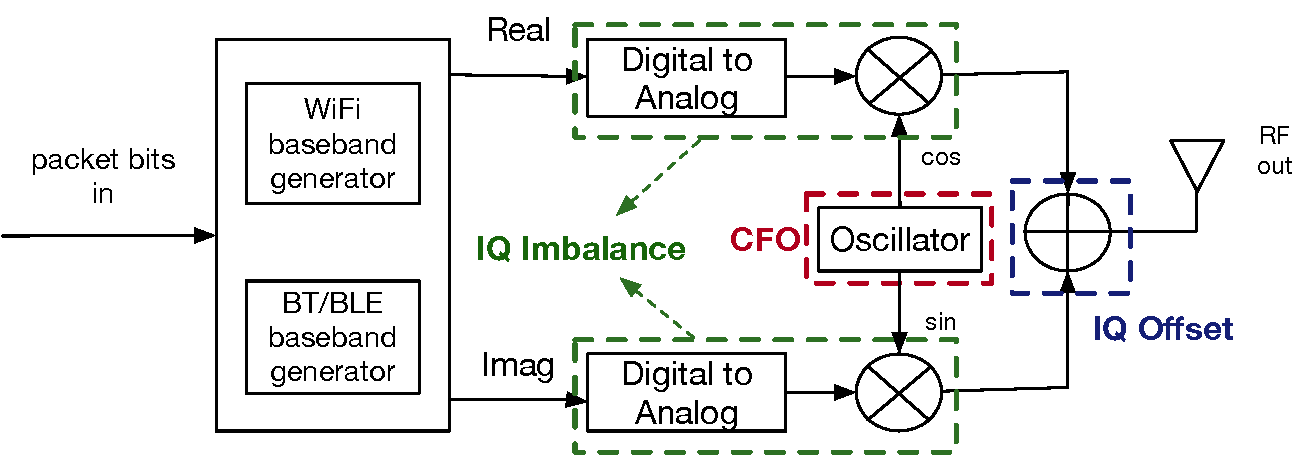
\includegraphics[width = \linewidth]{plots/IQchain.pdf} 
    \caption{Architecture of WiFi/BLE combo chipsets}
    \label{fig:iq_arch}
\end{figure}


WiFi chipsets have a unique fingerprint because they require generation of
complex multi-carrier modulation waveform. To generate this waveform, many
mobile device chipsets use an I/Q modulation architecture shown in
Figure~\ref{fig:iq_arch}.
%
The hardware imperfections in the I/Q architecture include the following:
\emph{Carrier Frequency Offset (CFO)} and \emph{IQ imperfections} (which
consists of IQ offset and IQ imbalance). \emph{CFO} is the error in the carrier
frequency fed to the mixer. It is caused by imperfections in the radio's
crystal oscillator; specifically, the crystal and the tolerance of oscillator
yields unique CFO even for the devices from the same make and model.
%
The \emph{IQ imperfections} result from the following phenomenon: IQ offset
comes from the center carrier leaking into the signal, or the baseband signal having a
DC offset.% This can add a fixed complex term to the I and Q sample (shift the
%center of constellation).
IQ imbalance occurs because of a mismatch
between parallel analog components of RF chain in I (in-phase) and Q
(quadrature) signal path.% This makes the phase and amplitude of I and Q path
%asymmetric. 

%In this type of
%transmitter, the I (real) and Q (imaginary) parts of the waveform are generated
%by the digital baseband. The real and imaginary parts of the signal are
%eventually mixed with a carrier frequency ($f_c$), where real part is
%multiplied cosine ($cos(2\pi f_c t$) of the carrier frequency and vice versa
%for imaginary part.

\subsubsection*{Mobile devices use combo BLE/WiFi chips}
%
In order to save the cost of RF hardware, high power devices (e.g. smartphones) are
equipped with combo chips which have both BLE and WiFi digital baseband, and
share the same I/Q front-end 
(Figure~\ref{fig:iq_arch}).
%
Combining these protocols reduces the device's overall size, and serves as a
point to synchronize both protocols' 2.4~GHz transmissions so they do not
interfere with each other.
%
However, an unintended result of this hardware design choice, is that BLE
transmissions contain the same imperfections that have been previously exploited to fingerprint WiFi transmitters.


%}}}

\subsection{Estimating CFO\&I/Q imperfections in BLE} %{{{
\label{sec:methodology1}

%
%These hardware imperfections have been demonstrated to be the most important
%characteristics for building RF fingerprinting systems for WiFi devices.  As a
%result, we can take advantage of these previously explored hardware
%imperfections to build our physical layer attack on BLE devices.
%
Although combo chips introduce WiFi-like imperfections in BLE transmissions
from mobile devices, estimating these imperfections in a capture of a BLE
transmission is extremely challenging (Section~\ref{sec:motivation:diff}).
%
%There is no existing technique for estimating the mentioned imperfections for
%BLE devices with the granularity and accuracy which is needed for the task of
%device identification.
%
%
First, we describe how typical BLE receivers perform limited, coarse grained,
estimation of physical-layer imperfections.
%
Then we present a new BLE fingerprinting algorithm that can estimate these
imperfections accurately and robustly, which is a requirement for the device identification attack.

%As discussed in Section~\ref{sec:background}, CFO, IQ offset and IQ imbalance
%are important hardware characteristics that can be leveraged to uniquely
%identify this architecture as proposed by prior works for fingerprinting WiFi
%devices as well. However, the challenge is how we can estimate these
%imperfection parameters accurately and fine-grained to fulfill the device
%identification task. WiFi signal eases this job by having specific signal
%features such as LTF and multiple subcarriers (and also WiFi chipsets report
%CSI which can easily be used to estimate these imperfections). This is mainly
%because fine-grained estimation and compensation of CFO and IQ imperfections is
%an unavoidable step in decoding WiFi signal. If CFO compensation is not
%accurate in WiFi decoding, IQ samples will rotate by time, and if IQ
%imperfection is not compensated, the shape of constellation will change. Both
%of these will drastically affect the decoding process since symbols are
%modulated in IQ domain. As a result, the mentioned signal features have been
%anticipated and there is a huge body of work on how to etimate these
%imperfections accurately for WiFi signals (not only for RF fingeprinting, but
%also for other purposes).


%In order to build a robust algorithm, we would start from the physics of the
%BLE architectures and build algorithms to capture hardware impariments to
%uniquely identify each radio. We present a novel algorithm to recover the
%hardware impairments which WiFi based RF fingerprinting relies on.
%Specifically, we would discuss how to extract the accurate hardware
%impairments such as CFO, IQ offset and IQ imbalance with just using the BLE
%transmissions which have narrow bandwidth with short packet sizes and short
%preamble length. 

%Next, we un-cover that not all devices use IQ architecture or popular architecture used by WiFi transceivers. In order to reduce power, the  reveal that BLE-only chipsets do not use the commonly known transmitter architecture and consequently, do not have many of the well-known hardware impairments. As a result, we porpose a new technique for profiling those architectures. Finally, we illustrate the overall flow of our fingerpriting methodology.
\begin{comment}
and we show that the second technique can be used to fingerprint any kind of bluetooth transmitter, regardless of the transmitter architecture.
\end{comment}

%Hardware Impairment estimation for WiFi/BLE Combo-chips}

% Talk about the combo chip first and explain how smartphone use those and therefore we can use the similar hardware impariments as IQ chipsets.

% this sentence says everything in one sentence slow it down, talk about WiFi devices first, show a figure with the architecture of the WiFi chipset to explain

%Practical hardware concerns have made the usage of I/Q path in transmitter architecture including WiFi chipsets, a desirable choice. In this kind of architecture, I and Q data are generated in different paths and eventually they are mixed with the carrier frequency. On the other hand, the hardware imperfections caused by this kind of hardware design, including CFO, IQ offset and IQ imbalance [CITE], have been proposed as important hardware characteristics which can be used to distinguish different devices. Naturally, the devices equiped with both BLE and WiFi technology (e.g. smartphones), utilize the same piece of hardware as a combo chipset for sending both BLE and WiFi packets as shown in Fig. XXXX. The reason lies in cost efficiency, simplifying board design, and optimizing die size and on-board area. As a result, we can take advantage of previously explored hardware imperfections (CFO, IQ offset and IQ imbalance). \\

%In previous works, CFO, IQ offset and IQ imbalance [CITE] have been proposed as important hardware characteristics which can be used to distinguish different devices. 


% Next talk about WiFi decodes the CFO etx and how it does, can we apply similar technique to BLE, we cannot, why?
% talk about how BLE is challenging with narrow bandwidth, short preamble makes it hard to detect CFO, if similar techqnieu as WiFi is applied what is the resolution you would get and would it resolve the devices (make the problem look hard)

%Measuring these harware imperfections is an unavoidable stage in decoding WiFi packets since it can significantly affect the decoding error if the receiver does not compensate them. As a result, measuring these imperfection has been heavily researched for WiFi signals. More than that, pecific arrangements have been devised in WiFi protocol to make the estimation of these imperfections easy and accurate. On the other hand, decoding the simple GFSK modulation which is used in BLE and Bluetooth, is not affected by the aforementioned imperfections severly. Therefore, there has not been any attempt on measuring these impairments accurately for a BLE or Bluetooth signal. Also, using the same techniques for estimating impairments as WiFi, will result in a much lower accuracy of estimation because of having a narrowband (without subcarrier) short signal (typically a few hundreds of microseconds) with a very short premble (8 microseconds). For instance, we employed the technique that is used in Bluetooth test equipments which exploits the preamble to estimate CFO [CITE]. That is, simply we take the average of frequencies in the preamble. Since preamble is an 8-bit sequence of consecutive 0 and 1, the frequency of preamble is symmetric. Therefore, ideally the average of thh frequencies in preamble must be 0. If there exists CFO, this average will be an estimate of CFO. However, this estimation is not precise and robust as it only relies on a an 8-microsecond preamble. The resulting standard deviation of the measured CFO was 1.5 KHz (we averaged the CFO standard deviation across 20 different devices). This standard deviation is huge for performing the task of RF fingeprinting and will end up in low accuracy of identifying devices based on RF fingerprints. We also tried the MINMAX algorithm described in [CITE] but it yields even worse standard deviation.\\

% then propose your solution layer by layer, first layer to increase the resolution your idea is to use entire packet, which requires you to decode the data and then reconstruct the receive singal witout hardware impariment and use that to estimate the impariements. 

%In WiFi it is necessary 
%features such as LTF and multiple subcarriers (and also WiFi chipsets report
%CSI which can easily be used to estimate these imperfections). This is mainly
%because fine-grained estimation and compensation of CFO and IQ imperfections is
%an unavoidable step in decoding WiFi signal. If CFO compensation is not
%accurate in WiFi decoding, IQ samples will rotate by time, and if IQ
%imperfection is not compensated, the shape of constellation will change. Both
%of these will drastically affect the decoding process since symbols are
%modulated in IQ domain.

% Extra text {{{
\if 0
Unlike WiFi, decoding BLE or Bluetooth signals does not require accurately
estimating and compensating for CFO and IQ imperfections.
%
Even several KHz of CFO will not affect the decoding process of BLE's FSK
signals. Also, as FSK symbols are not modulated in IQ domain, IQ imperfections
does not significantly the affect BLE decoding process.
%
As a result, unlike WiFi, there was no need to embed any known signal feature
in BLE signal to provide necessary means for accurate and fine-grained
estimation of these imperfections.
%
For instance, BLE preamble is only 8 bits (8 microseconds) which is much
shorter than WiFi, it uses the simple GFSK modulation, and there does not
exists multiple subcarrier in BLE signal or CSI in BLE chipsets. These
simplicities of BLE signal leaves us in a situation where estimating these
imperfections for BLE signals is much more challenging than WiFi.
The consequence of this fact is that existing techniques for fine-grained
estimation of CFO and IQ imperfection of WiFi signals, either cannot be
adopted or will not result in fine-grained imperfection estimation for BLE
signals.  Moreover, techniques that are specifically designed for CFO
estimation of BLE or Bluetooth signals provides only a very coarse-grained
estimation which is not sufficient for device identification task at all, and
not surprisingly, there has not been any attempt on estimating IQ imperfection
for BLE or BLuetooth signals as it is not needed for decoding.
\fi
%}}}

\vspace{0.5em}
\noindent\textbf{Existing coarse CFO estimation methods in BLE receivers}
Coarse-grained CFO compensation is implemented in BLE receivers.  They
implement this by analyzing the small number (8) of known samples in the
preamble of each packet.
%
BLE receivers estimate CFO from these bits by averaging the frequencies of each
FSK symbol in the preamble. Another popular CFO algorithm used in the Texas
Instruments CC2400 BLE chipset averages the minimum and maximum frequency of
the preamble~\cite{cvtracksun}.
%
Since the preamble is an 8-bit sequence of consecutive 0 and 1, the frequency
of preamble is symmetric.  Therefore, ideally the average of the frequencies in
preamble must be 0. If there exists CFO, this average will be an estimate of
CFO.
%
However, as these techniques only rely on 8 samples in the preamble. Consequently, they do not produce an
accurate estimate of CFO---leading to confusions between device fingerprints.
%
Indeed, with only 8 samples, the theoretical limit of CFO accuracy 2 KHz assuming 3 degree phase noise. Moreover, inaccurate or coarse-grained compensation of CFO, significantly affects I/Q offset and imbalance estimation as it causes rotation of I/Q samples in I/Q constellation.



%

%
% ADS: Sounds fun but no space
%
%We tried simply extending this method to take advantage of the entire packet
%and take average across frequencies of equal number of 0's and 1's. However,
%we did not see any significant benefit for doing that.

\subsubsection{Goals}
%
To implement an improved BLE RF fingerprinting algorithm, and to estimate I/Q
in addition, our algorithm must have two key properties.
%
First, instead of relying on the 8 known samples in the preamble, our goal is
to utilize the entire packet ($\sim$370 samples).
% in order to diminish the
%effect of noise and provide more information and granularity for accurate
%imperfection estimation.
These additional samples will provide a theoretical CFO accuracy of 
11 Hz compared to the 2 KHz of coarse-grained
estimation.
%
Second, it must jointly estimate CFO and I/Q imperfections to prevent the
mutual effects on each other's estimation.

\subsubsection{Overview}
%
Keeping these two goals in mind, we develop an algorithm to estimate CFO and IQ
imperfections for BLE signals.
%
To be able to take advantage of the entire packet properly, we need to first
decode the packet. Our insight is that because GFSK modulation is robust to CFO, IQ imperfections and noise,
we will be likely to decode the packet correctly, and this can be checked with
BLE's CRC.
%
Once we have the decoded data, we can reconstruct an ideal perfect version of
the transmitted signal.
%
Then we jointly insert the hardware imperfection parameters (CFO and I/Q) in the
mathematical model of the ideal signal. Then we keep modifying those
imperfection parameters until the representation of the signal
looks like the actual captured signal. However, since the search space for
these imperfection parameters is vast, we use optimization techniques to
efficiently move towards the optimal value of parameters.

%to WiFi. Therefore, decoding can be done properly without compensating hardware
%imperfections.  

%However, to build an algorithm for estimating these fingerprints accurately and robustly, despite the existing techniques, we cannot rely on the preamble since it is very short for BLE and also, there is no notion of subcarrier in BLE technology. For instance, we employed the technique that is used in Bluetooth test equipments which exploits the preamble to estimate CFO~\cite{?}. That is, simply we take the average of frequencies in the preamble. Since preamble is an 8-bit sequence of consecutive 0 and 1, the frequency of preamble is symmetric. Therefore, ideally the average of the frequencies in preamble must be 0. If there exists CFO, this average will be an estimate of CFO. However, this estimation is not precise and robust enough as it only relies on a an 8-microsecond preamble. The resulting standard deviation of the measured CFO was 1.5 KHz (we averaged the CFO standard deviation across 20 different devices). This standard deviation is huge for performing the task of RF fingeprinting and will end up in low accuracy of identifying devices based on RF fingerprints. \\

%Instead of relying on preamble or specific short parts of the packet, we can benefit from the entire packet to make a robust and accurate imperfection estimator since using the entire packet helps in diminishing the effect of noise as well as providing more information and granularity to estimate imperfections accurately. Although for being able to take advantage of the entire packet properly, we need to first decode the packet. Note that thanks to simple GFSK modulation, hardware imperfection does not cause decoding error as opposed to WiFi. Therefore, decoding can be done properly without compensating hardware imperfections. Once we have the decoded data, we can reconstruct the ideal signal. The high level idea is that we insert hardware imperfection parameters in the mathematical model of the ideal signal. Then we keep changing those imperfection parameters until the mathematical representation of the signal looks like the actual captured signal. However, since the search space for these imperfection parameters is vast, we use optimization techniques to move towards the optimal value of parameters efficiently. \\
%Although we consider GFSK modulation in this paper, the idea behind this method can be extended to many other modulation schemes. 

% estimating impariments is not easy, explain the math model and explain why it is hard, as it not convex 

% present your insights to use a gradient descent algorithm, however even that gets stuck at local minima's which is not great, so you fix this by choosing right intial value. 

% explain how you choose right initial value, what are your insgihts and why does those work. 

% finally show the performance of your algorithm before ending the section. 




\begin{comment}
    To measure these hardware impairments, we mathematically model them and then use optimization techniques to estimate these imperfections. 
\end{comment}

\subsubsection{Jointly estimating CFO and I/Q}
\begin{figure}[t!]
    \centering
    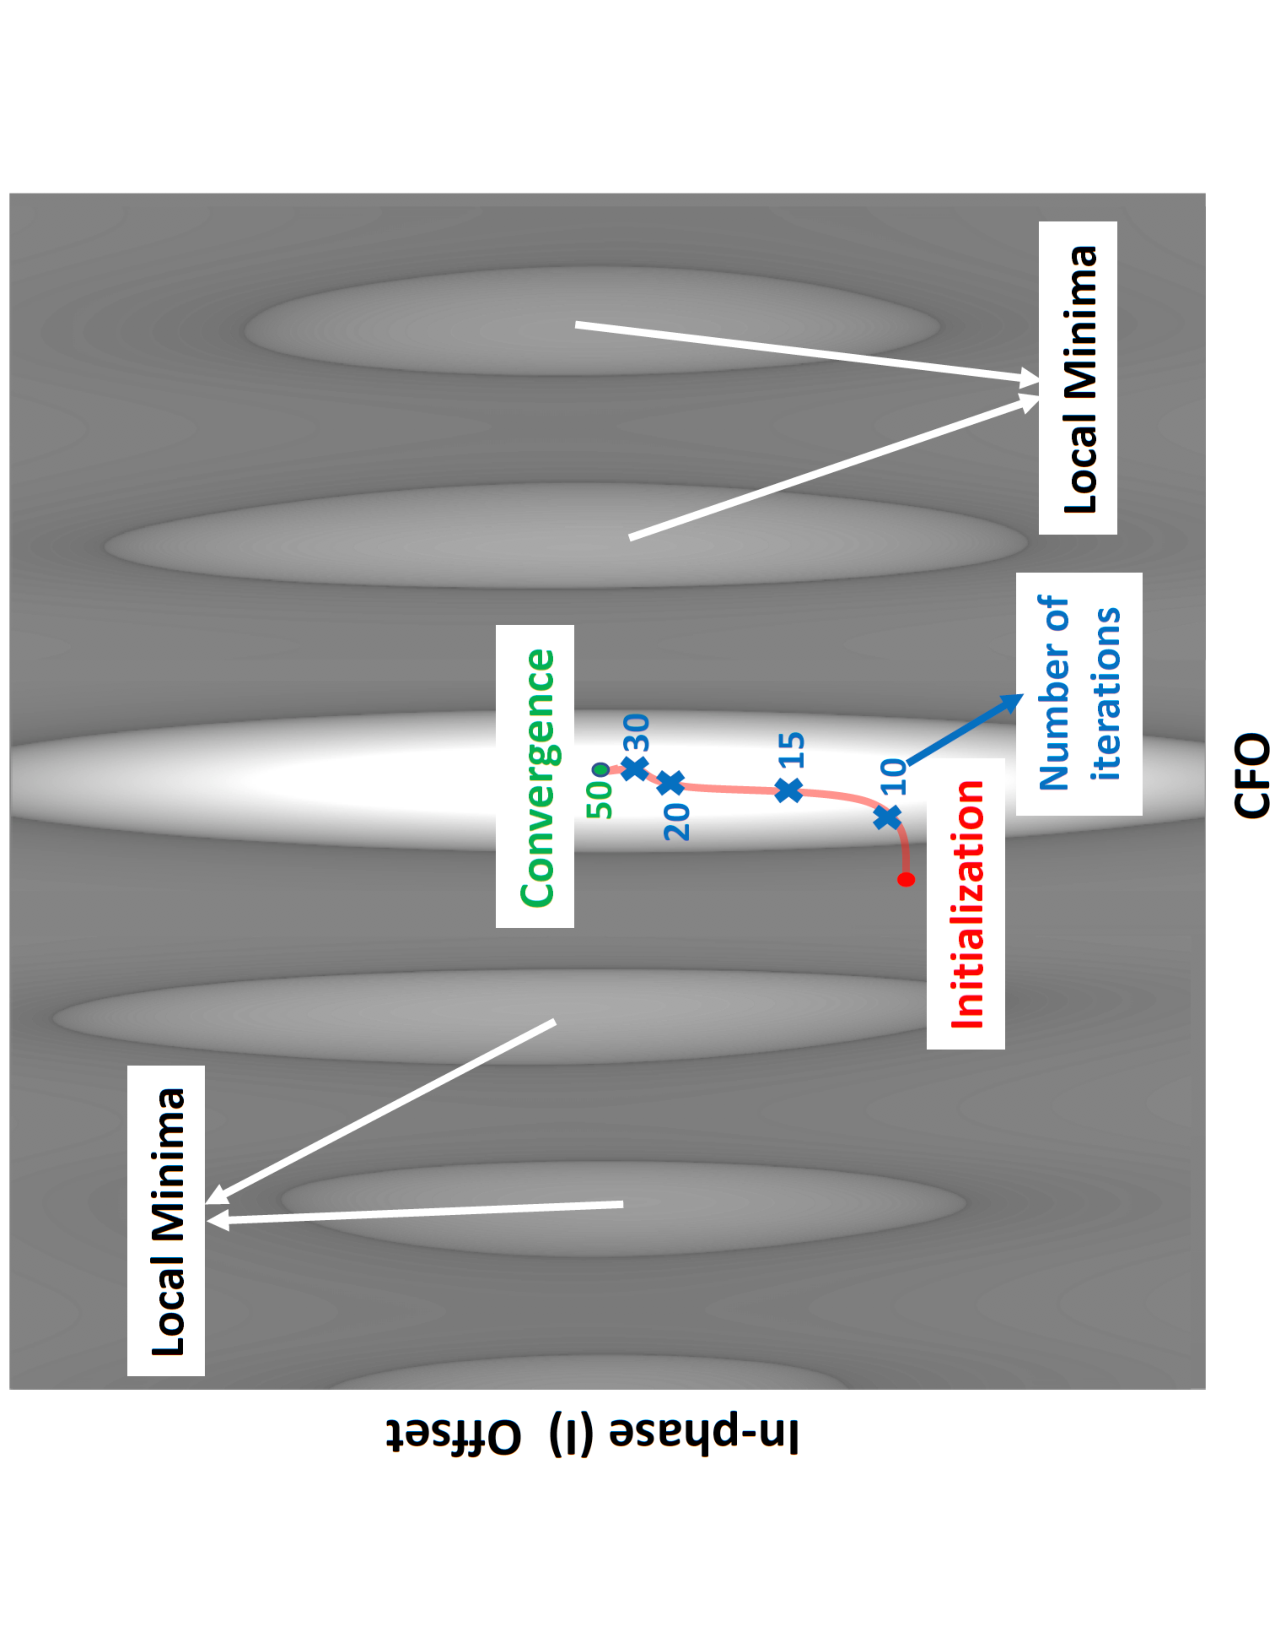
\includegraphics[angle = 270, width = \linewidth]{plots/heatmap.pdf} 
    \caption{Visualization of how the optimization based algorithm converges to the accurate hardware imperfection values such as CFO and IQ offset.}
    \label{fig:heatmap}
\end{figure}
Let $y = Real\{y\}+jImag\{y\}$ be the captured baseband signal (normalized by the average amplitude). In a GFSK modulated signal, ideally we have $Real\{y\} = cos(\omega(t)t)$ and $Imag\{x\} = sin(\omega(t)t)$ where $\omega(t)$ is the baseband frequency of the signal which is generated according to the GFSK modulation. However, the aforementioned hardware imperfections will slightly change the signal. We first decode the signal to obtain the sequence of bits and then, we make $\omega(t)$ according to GFSK modulation. Let $y'$ be the model of the imperfect signal. Considering the effects of CFO, IQ offset and IQ imbalance, we can write
\begin{gather*}
    y'(t) = \big[(A-\frac{\epsilon}{2})cos(\omega(t)t-\frac{\phi}{2})+I+ \\
    j\big((A+\frac{\epsilon}{2})sin(\omega(t)t+\frac{\phi}{2})+Q)\big)\big]e^{j(\phi_o+2\pi f_o t)}
\end{gather*}
where $f_o$, $\phi_o$, $A$, $\frac{\epsilon}{A}$, $\phi$, $\frac{I}{A}$ and $\frac{Q}{A}$ denote CFO, phase offset, normalized amplitude of the signal, IQ amplitude imbalance, IQ phase imbalance, I offset and Q offset, respectively. The goal is to choose the value of these variables in such a way that $||y'-y||^2$ is minimum and as a result, $y'$ is as close as possible to the captured signal $y$. Therefore, we must solve the following optimization problem:
\begin{gather*}
    min_{f_o,\phi_o,A,\epsilon,\phi,I,Q}{F=||y'-y||^2 =} \\ |Real\{y'\}-Real\{y\}|^2+|Imag\{y'\}-Imag\{y\}|^2
\end{gather*}
However, this problem is not convex and the objective function has several local minimas as shown in Figure~\ref{fig:heatmap}. Consequently, any optimization technique may end up in a local optima. To avoid this, we initialize the variables properly to increase the chance of finding the global minimum significantly. Although theoretically it will not guarantee ending up in the global minimum for arbitrary optimum numbers of these variables, we found that in practice we will reach the optimum value with this initialization in practical conditions. 

To initialize CFO, start by taking the average of frequencies in the preamble. Then we compensate the initial CFO in the signal to get the signal $z = y e^{-2\pi f_o t}$. To estimate initial I/Q imperfections, we use the I/Q constellation of the GFSK signal. The I/Q constellation of an ideal GFSK signal is a circle centered at $(0,0)$ since the phase changes according to GFSK modulation but the amplitude is always constant. However, I/Q imperfection will change this constellation. Specifically, I/Q offset will shift the center of the circle as it is equivalent to adding a fixed complex term to the ideal signal, and IQ imbalance will change the shape from a circle to a tilted ellipse.
%
%These effects are shown in Figure~\ref{fig:iq_const}.
As a result, to get an initial estimation of IQ imperfections, we fit an ellipse to the 2-dimensional points $(Imag\{z\},Real\{z\})$ by minimizing the Least Square Error. The center of the ellipse will provide the initial IQ offset and initial IQ imbalance can be obtained from the ratio of minor and major diameter and rotation angle of the ellipse.\\

\if 0
\begin{figure}[t!]
    \centering
    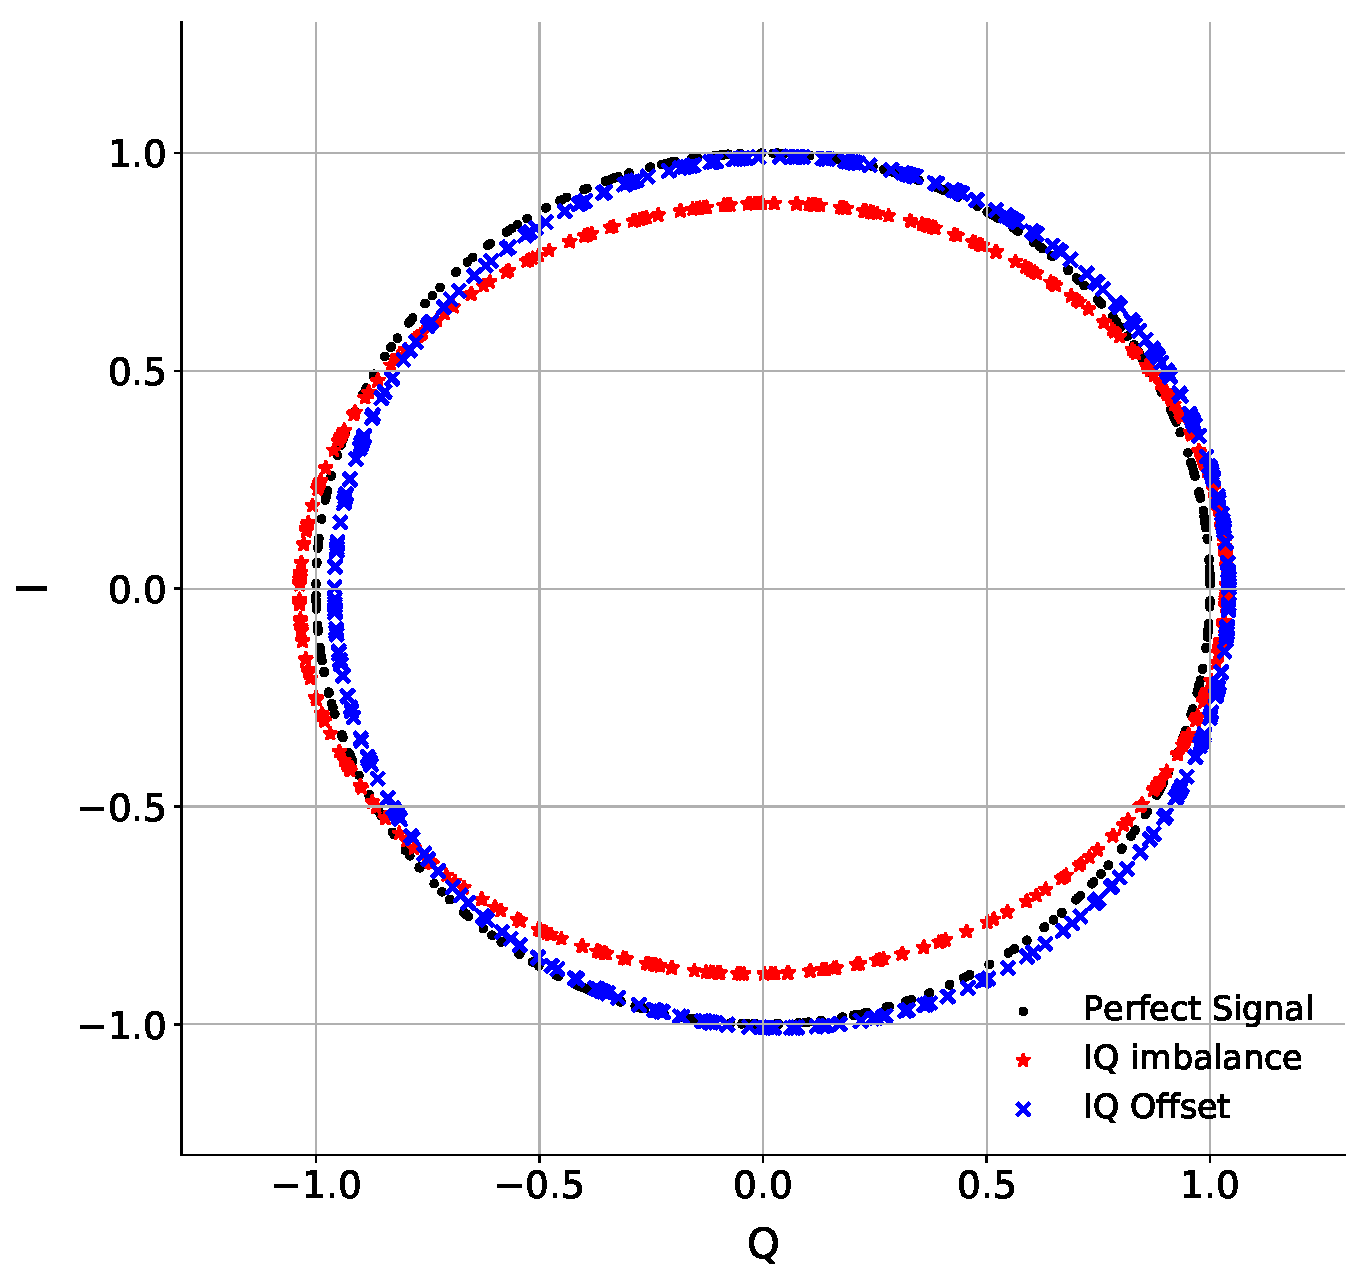
\includegraphics[width = \linewidth]{plots/IQ_const.pdf} 
    \caption{Effects of IQ imperfection on IQ constellationo of a GFSK signal without noise and CFO}
    \label{fig:iq_const}
\end{figure}
%it will be long if I want to explain this ellipse thing
\fi

Although, these initial estimations provide an initialization close to optimum,
they are not accurate. As mentioned earlier, this initialization of CFO
is not accurate and robust enough as it only relies on an 8-microsecond
preamble. Also, mismatch in CFO compensation will cause a time-dependent phase
shift which distorts the I/Q constellation. Therefore, the initial IQ offset
and imbalance estimation will also have errors. Consequently, we employ
optimization techniques to jointly estimate hardware imperfection parameters
precisely and robustly. Therefore, after this initialization, we use Nesterov
Accelerated Gradient Descent (NAG) to move from the initialization towards the optimum values
of $f_o,\phi_o,A,\epsilon,\phi,I,Q$ by minimizing $F$ in the mentioned
optimization problem. Figure~\ref{fig:heatmap} demonstrates an instance of how we start from the initial estimations of CFO and IQ imperfections, move toward the optimal values of CFO and IQ imperfections using gradient descent (the red line), and converge to the accurate estimations of CFO and IQ imperfections.

% TOO LONG ====================
%However, as mentioned earlier, this optimization problem is convex and we may converge to the local optima. Therefore, if after convergence, the average of $F$ was not less than a certain threshold which is determined according to SNR, we add certain steps to the first initialization and repeat the aforementioned gradients descent process. We keep searching for the optimum with new initializations until either the average of $F$ falls below the threshold or our initialization falls out of the bound of the typical values for these imperfections (in which case we give up on the packet. This typically happens when the SNR is less than 5 dB or there is a collision). The first initialization will increase the speed of convergence as usually it will be close to the optimum and re-initialization will ensure ending up in a point which is either the global optimum or very close to global optimum (in the sense that the objective function is less than the desired threshold and hence, is within a small margin of global optimum). The proposed algorithm fulfills the two key properties that we explained at the beginning of this subsection. First, the NAG based joint estimation of CFO and IQ imperfections ensures precise estimation with fine granularity as it keeps moving towards the optimum with adaptive steps and removes the mutual effect of mismatch in estimating these imperfection parameters. Second, the objective function of optimization is chosen as the summation of all PHY samples across the packet, which diminishes the impact of AWGN and provide more robust information and granularity. The final result is achievement of a highly precise CFO and IQ estimates for a device, that are robust to environmental noise, and can therefore be used by an attacker as a unique fingerprint for generic consumer devices.
% Shorter ==========
However, as mentioned earlier, this optimization problem is not convex and we may converge to the local optima. Therefore, if after convergence, the average of F was not less than a certain threshold which is determined according to SNR, we add certain steps to the first initialization and repeat the aforementioned gradients descent process. The proposed optimization based estimation ensures precise estimation with fine granularity as it keeps moving towards the optimum with adaptive steps and removes the mutual effect of mismatch in estimating these imperfection parameters. Moreover, the objective function of optimization is chosen as the summation of all PHY samples across the packet, which diminishes the impact of AWGN and provide more robust information and granularity.

% This is restated, so cutting other eval is there now
\if 0
We use this methods to extract CFO, IQ offset and IQ imbalance for 20 ESP32 chipsets of the same make and model. Figure~\ref{fig:esp} represents CFO and IQ offset magnitude for 10 packets for each of these 20 chipsets. The low variance of CFO for each device, shows this methods is very precise in measuring hardware imperfections (e.g. the CFO standard deviation average for 20 devices is 200 Hz in our algorithm which is significanly less than the existing methods described earlier). Obviously, low within-class variance will significantly improve the identification accuracy and these 20 devices can be clearly distinguished only by their CFO and IQ offset. 
\fi

\vspace{0.5em}
\noindent\textbf{Summary:} For the first time we showed that it is feasible to estimate CFO and IQ imperfections of WiFi/BLE combo chipsets based on the simple BLE signal itself; in other words, without needing the rich signal features that are present in WiFi.


\subsubsection{Profiling and identifying the device}
\label{sec:methodology2}

The first step in deploying our RF fingerprinting attack is to capture the BLE signal. We use an SDR to capture raw I and Q samples of BLE. Next, we use the captured signal to fingerprint the device. The entire processing flow can be divided into two stages, Fingerprinting Stage and Identification Stage. In the former stage, the device is isolated and we capture a number of packets from the target device to build a profile for the device (training packets). The latter stage, employs this profile to identify the device when the MAC addresses is changed.

\vspace{0.5em}
\noindent\textbf{Fingerprinting Stage:} For each packet from a device $D$, CFO and IQ imperfections can be extracted with a high resolution using algorithm described in~\ref{sec:methodology1}. Let $x_1,...,x_N$ be the CFO and IQ imperfection feature vectors for $N$ training packets we have received from device $D$. We calculate the mean $\mu_D$ and covariance matrix $\Sigma_D$ of $X = [x_1 \quad ... \quad x_N]$. $\mu_D$ and $\Sigma_D$ together with a threshold that will be defined later is considered the profile of device $D$.

\noindent\textbf{Identification Stage:} In identification stage, we want to decide whether a packet $x_t$ with a new MAC address belongs to device $D$, indicating that the target device is present. To do so, we compute the Mahalanobis distance to the profile of device $D$

\begin{gather*}
    distance(x_t,\mu_D,\Sigma_D) = \sqrt{(x_t-\mu_D)^T\Sigma_D^{-1}(x_t-\mu_D)}
\end{gather*}


This distance is a way to measure how close the features of the new packet are to the profile of device $D$. In addition to $\mu_D$ and $\Sigma_D$, we define a threshold $thresh$ as the profile of the device. Whenever $distance(x_t,\mu_D,\Sigma_D)<thresh$, packet $x_t$ belongs to the target device $D$ and device $D$ is identified. Otherwise, packet $x_t$ belongs to some other device in the world that we are not looking for. This threshold is chosen using the validation set.
Moreover, since the MAC address is fixed for a period of time, we receive a number of packets with the same MAC address which we know belong to the same device. As a result, we can make a decision about the identity of the MAC address instead of the individual packets. One way that we found most effective, was to first average the feature vector $x$ for all packets with the same MAC address and then compute the Mahalanobis distance. This would further reduce the tolerance due to estimation error and inherent tolerance of features.

\if 0 % extra {{{
\paragraph{Fingerprinting Stage} For each packet from a device $D$, CFO anf IQ imperfections (IQ offset and IQ imbalance) can be extracted with a high resolution using algorithm described in~\ref{sec:methodology1}. Let $x_1,...,x_N$ be the CFO and IQ imperfection feature vectors for $N$ training packets we have received from device $D$. We calculate the mean $\mu_D$ and covariance matrix $\Sigma_D$ of $X = [x_1 \quad ... \quad x_N]$. $\mu_D$ and $\Sigma_D$ together with a threshold that will be defined later is considered as the profile of device $D$.



%Note that IQ offset and imbalance are only useful for combo transmitters and will be ignored by classifier while classifying BLE-only transmitters.
\paragraph{Identification Stage} In identification stage, we want to decide whether a packet $x_t$ with a new MAC address belongs to device $D$, indicating that the target device is present. To do so, we compute the Mahalanobis distance to the profile of device $D$

\begin{gather*}
    distance(x_t,\mu_D,\Sigma_D) = \sqrt{(x_t-\mu_D)^T\Sigma_D^{-1}(x_t-\mu_D)}
\end{gather*}
\begin{gather*}
    distance(x_t,\mu_D,\Sigma_D) = \sqrt{(x_t-\mu_D)^T\Sigma_D^{-1}(x_t-\mu_D)}
\end{gather*}
%This is assuming that the estimated CFO and IQ imperfections have a Gaussian distribution which is a fair assumption considering that the tolerance in CFO and IQ imperfection estimation of a device for different packets is mainly caused by variations in SNR (which affects estimation error) and tolerance of the underlying hardwar.
This distance is one way to measure how close the features of the new packet are to the profile of device $D$. In addition to $\mu_D$ and $\Sigma_D$, we define a threshold $thresh$ as the profile of the device. Whenever $distance(x_t,\mu_D,\Sigma_D)<thresh$, packet $x_t$ belongs to the target device $D$ and device $D$ is identified. Otherwise, packet $x_t$ belongs to some other device in the world that we are not looking for. This threshold is chosen using the validation set.
Moreover, since the MAC address is fixed for a period of time, we receive a number of packets with the same MAC address which we know belong to the same device. As a result, we can make a decision about the identity of the MAC address instead of the individual packets. One way that we found most effective, was to first average the feature vector $x$ for all packets with the same MAC address and then compute the Mahalanobis distance. This would further reduce the tolerance due to estimation error and inherent tolerance of features.


\fi
%}}}

\subsubsection{Comparing CFO accuracy} %{{{
\begin{figure}[t!]
    \centering
    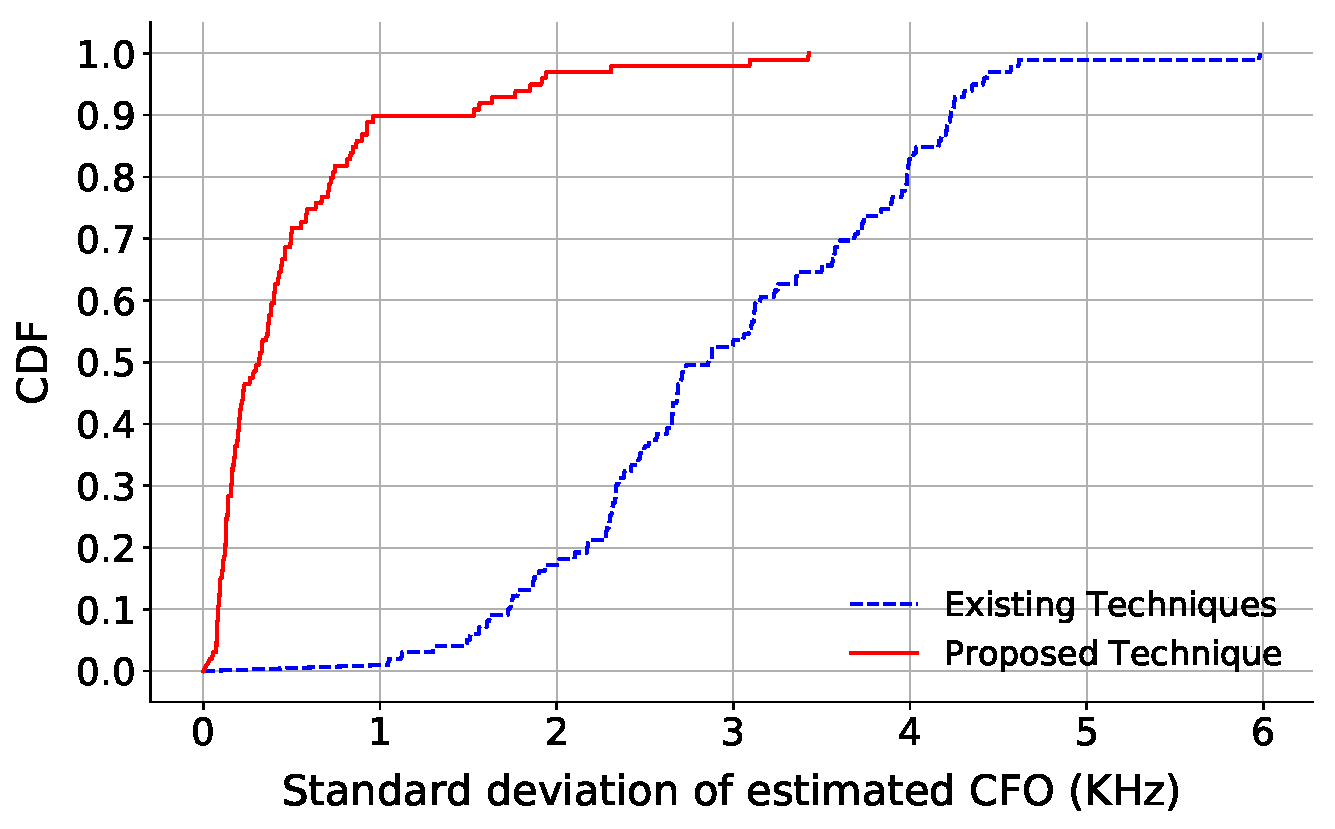
\includegraphics[width = \linewidth]{plots/CFO_comparison_ESP.pdf} 
    \caption{Comparing the CFO estimation of existing coarse-grained techniques with our proposed technique.}
    \label{fig:cfo_comp}
\end{figure}


%
To evaluate the accuracy of our new fine-grained fingerprinting algorithm compared to coarse-grained BLE
CFO estimation, 
we compute CFO for 100 packets from 100 of BLE transmitters observed in the field.% For each device, we
%consider the CFO estimation technique which yielded the lowest standard deviation (std).
%
Figure~\ref{fig:cfo_comp} shows the CDF of the standard deviation of CFO for both techniques.
%
We see that 
our fine-grained CFO estimation significantly reduced the standard deviation of CFO estimation for all devices. This reduces the within-class variance and
makes these devices have significantly more unique fingerprints.
%Moreover, as inaccurate estimation and compensation of
%CFO affects the estimation of IQ imperfections since the residual CFO will
%cause IQ samples to rotate by time.
% In fact, no prior work has
%demonstrated that it is possible to obtain accurate and identifiable estimates
%of imperfections for BLE transmitters.
%
%Consequently, we must develop a new
%algorithm to enable find-grained and robust estimation of CFO and IQ
%imperfections to enable our device identification attack.

%The resulting standard deviation of the measured CFO was 1.5 KHz (we averaged the CFO standard deviation across 20 different devices). This standard deviation is huge for performing the task of RF fingeprinting and will end up in low accuracy of identifying devices based on RF fingerprints. 
%}}}
